\documentclass[t, 10pt, handout, aspectratio=169]{beamer}
\usepackage{lipsum}
\usepackage{tikz}
\usepackage{pgfplots, pgfplotstable}
\usepackage{booktabs}
\usepackage{amsmath,bm,amstext}
\usepackage{mdframed}
\usepackage{mleftright}



\pgfplotsset{compat=1.14}

%\usetheme[framenumber,totalframenumber]{QU}
\usetheme[color=blue,framenumber,totalframenumber, footline, footertext]{KU}


\title[Introduction to Tensor]{Introduction to \texttt{Tensor}}
\subtitle{Intelligent Computing for Computational Intelligence \\
in post Moore’s Law era!}

\author[yanglet]{Xiao-Yang Liu\\
\url{www.tensorlet.com}}
\institute[CU]{Columbia University}

\footertext{\textcolor{red}{\url{www.tensorlet.com}}}


\date[\number\month/\number\day/\number\year]{\today}


\begin{document}

\begin{frame}
  \titlepage
\end{frame}

\begin{frame}{Agenda}
\begin{itemize}
    \large \item \textcolor{red}{Background}
    \large \item {Tensor Decompositions (CP, Tucker, and Tensor-Train/Tensor-Ring)}
    \large \item{Transform-based Tensor Model and Applications}
    \large \item{Tensor Computations (cuTensor, TensorDeC$++$)}
\end{itemize}
\end{frame}

\begin{frame}{Background}
~~In sensing systems, the number and resolution of the sensors grow to the point that multidimensional data of exceedingly huge volume, variety and structural richness become ubiquitous across disciplines in engineering and data science.
\begin{figure}
	\centering  
	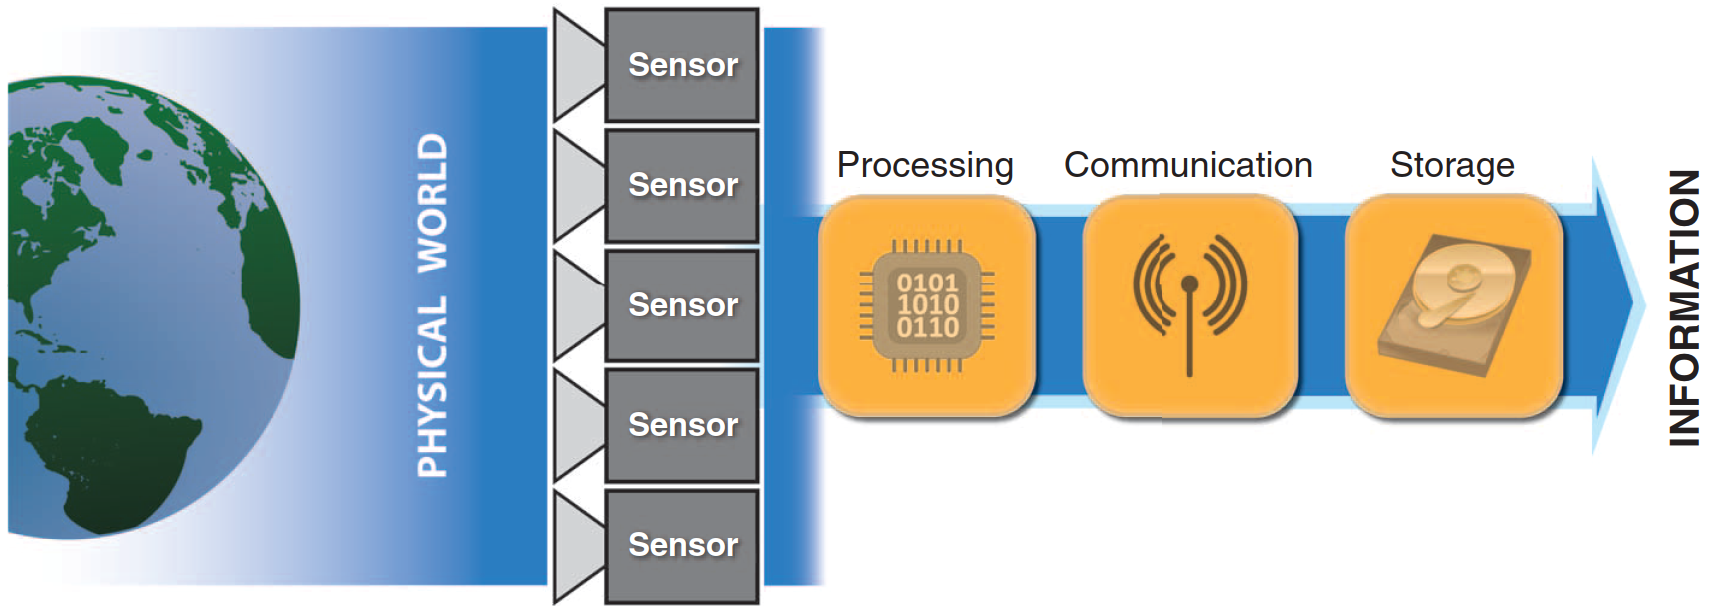
\includegraphics[width=\linewidth]{figs/data_deluge.png}
	\label{fig:data_deluge}
\end{figure}
\end{frame}

\begin{frame}{Background}
\begin{columns}
\column{0.55\linewidth}
~~Many problems in computational neuroscience, neuroinformatics, pattern/image recognition, signal processing and machine learning generate massive amounts of multidimensional data with multiple aspects and high dimensionality. These data have four ``V'' characters, as shown in the right figure.

~

~~\textbf{Tensor} provides a natural and compact representation for such massive multidimensional data via suitable low-rank approximations, of which the dynamic analysis allows us to discover meaningful hidden structures of complex data and to perform generalizations by capturing multi-linear and multi-aspect relationships. 
\column{0.5\linewidth}
\vskip -6.6ex
\begin{figure}
	\centering  
	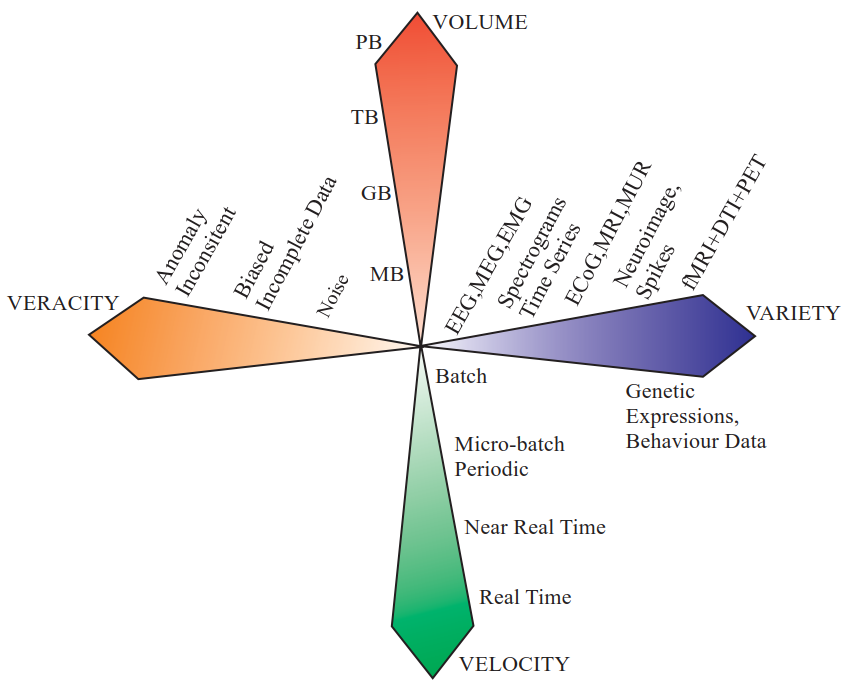
\includegraphics[width=0.95\linewidth]{figs/4v_characters.png}\\
	Volume - scale of data\\
	Variety - different forms of data\\
	Veracity - uncertainty of data\\
	Velocity - analysis of streaming data
	\label{fig:4v_characters}
\end{figure}
\end{columns}
\end{frame}

\begin{frame}{What Is Tensor?}
\vskip -1ex
\begin{figure}
	\centering  
	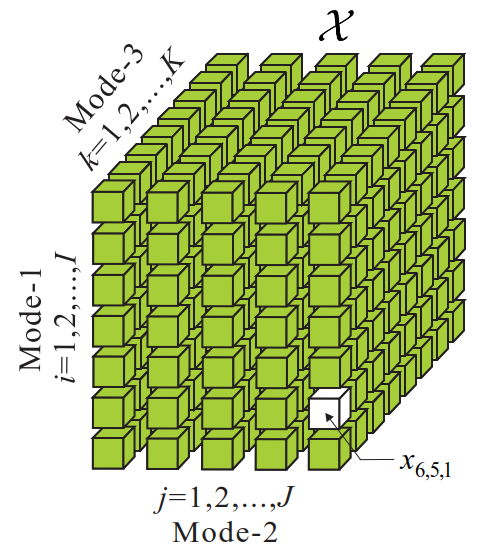
\includegraphics[height=0.7\paperheight]{figs/tensor_shape}
	\label{fig:tensor_shape}
\end{figure}
\end{frame}

\begin{frame}{What Is Tensor?}
\vskip -1ex
\begin{figure}
	\centering  
	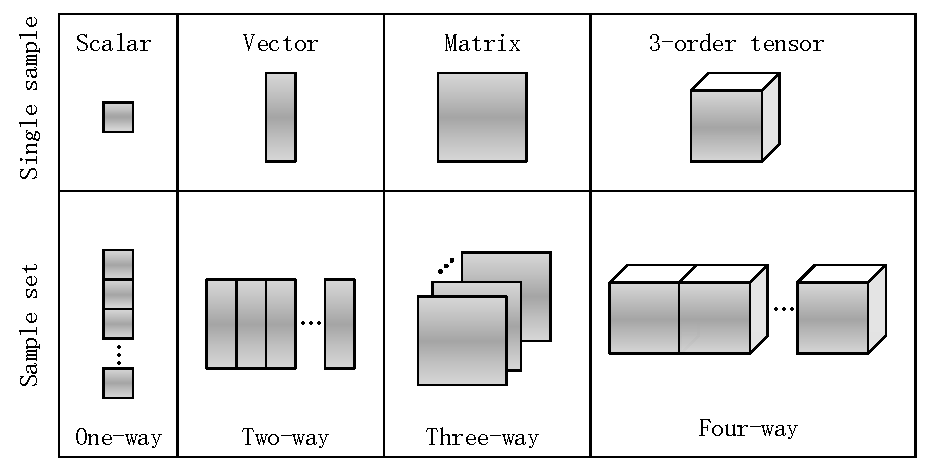
\includegraphics[height=0.7\paperheight]{figs/tensor_sample}
	\label{fig:tensor_sample}
\end{figure}
\end{frame}

\begin{frame}{Tensor Fibers}
\begin{figure}
	\centering  
	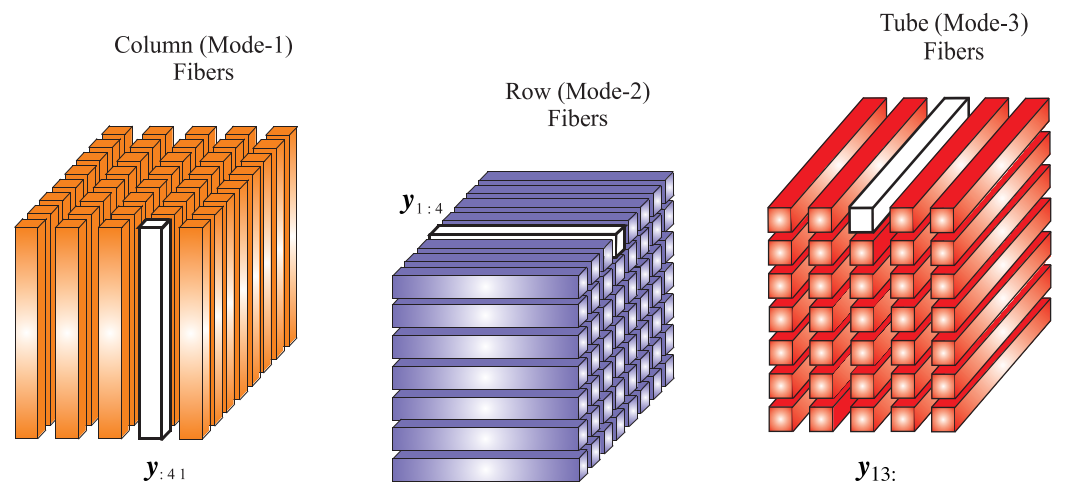
\includegraphics[width=\linewidth]{figs/tensor_fibers}
	\label{fig:tensor_fibers}
\end{figure}
\end{frame}

\begin{frame}{Tensor Slices}
\begin{figure}
	\centering  
	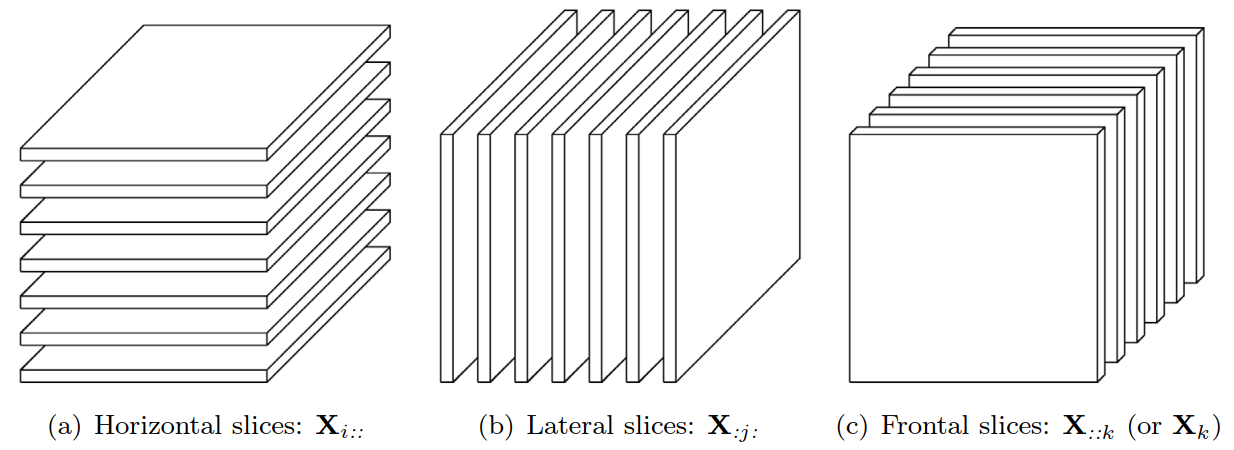
\includegraphics[width=\linewidth]{figs/tensor_slices}
	\label{fig:tensor_slices}
\end{figure}
\end{frame}

\begin{frame}{Tensor Unfolding}
\vskip -1ex
\begin{columns}[c]  %开始进入分栏环境,居中设置
\column{0.35\linewidth}  
\begin{figure}
	\centering  
	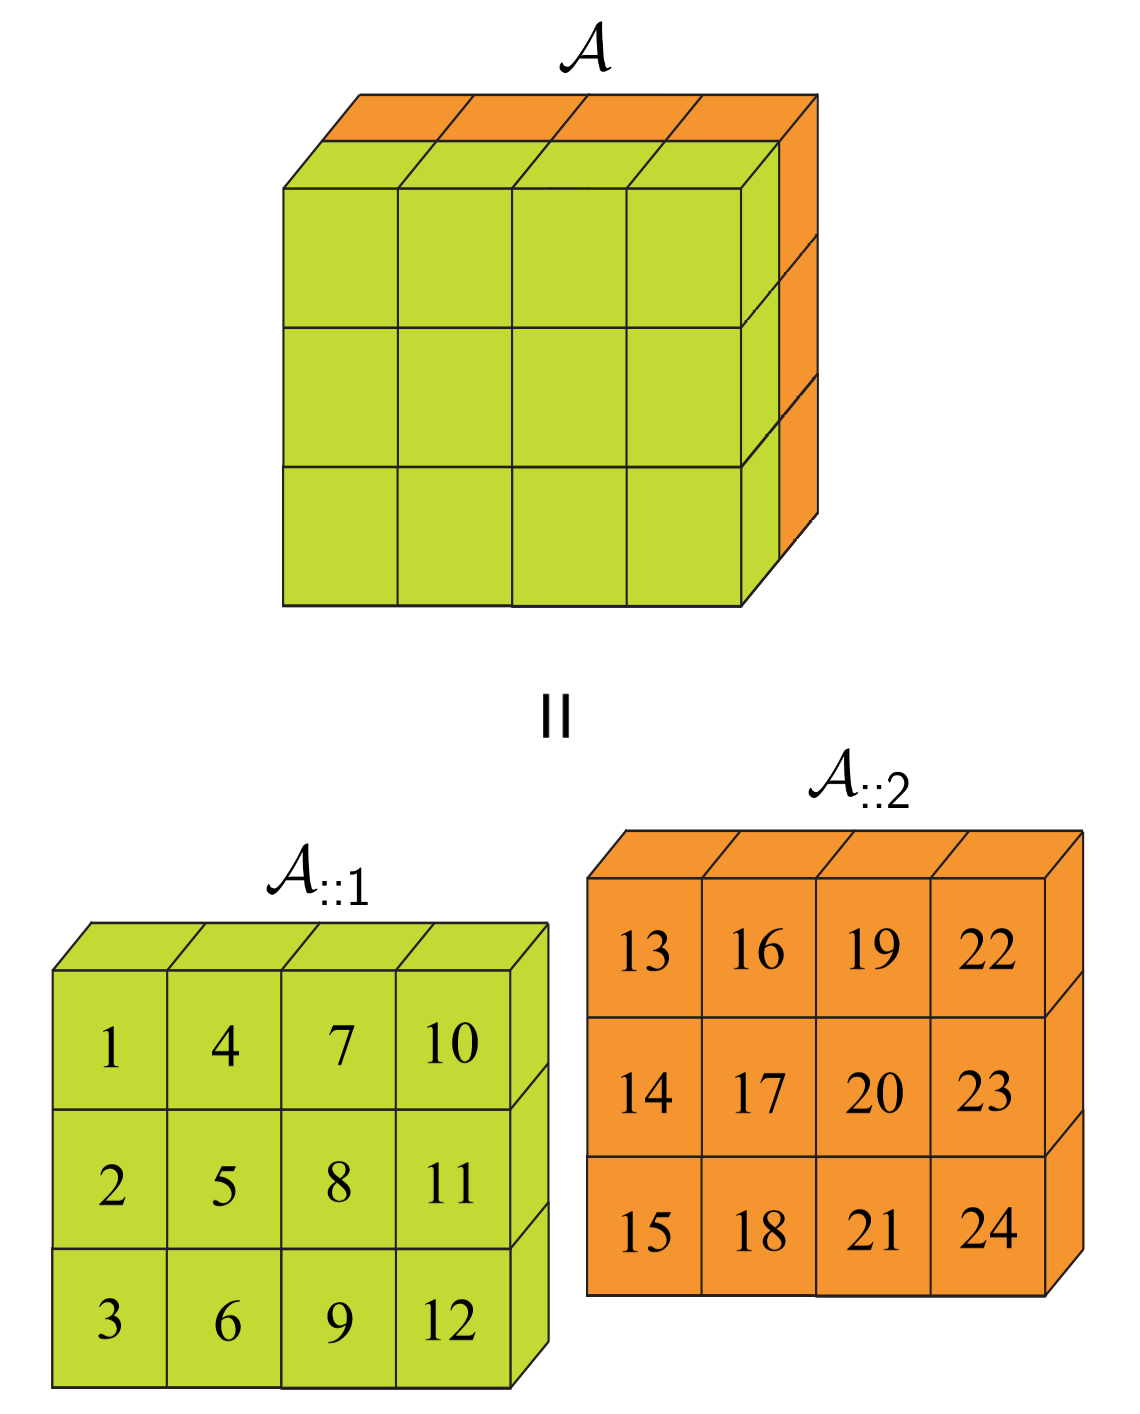
\includegraphics[width=\linewidth]{figs/tensor_unfolding1.png}
	\label{fig:tensor_unfolding1}
\end{figure}

\column{0.65\linewidth}  
\begin{figure}
	\centering  
	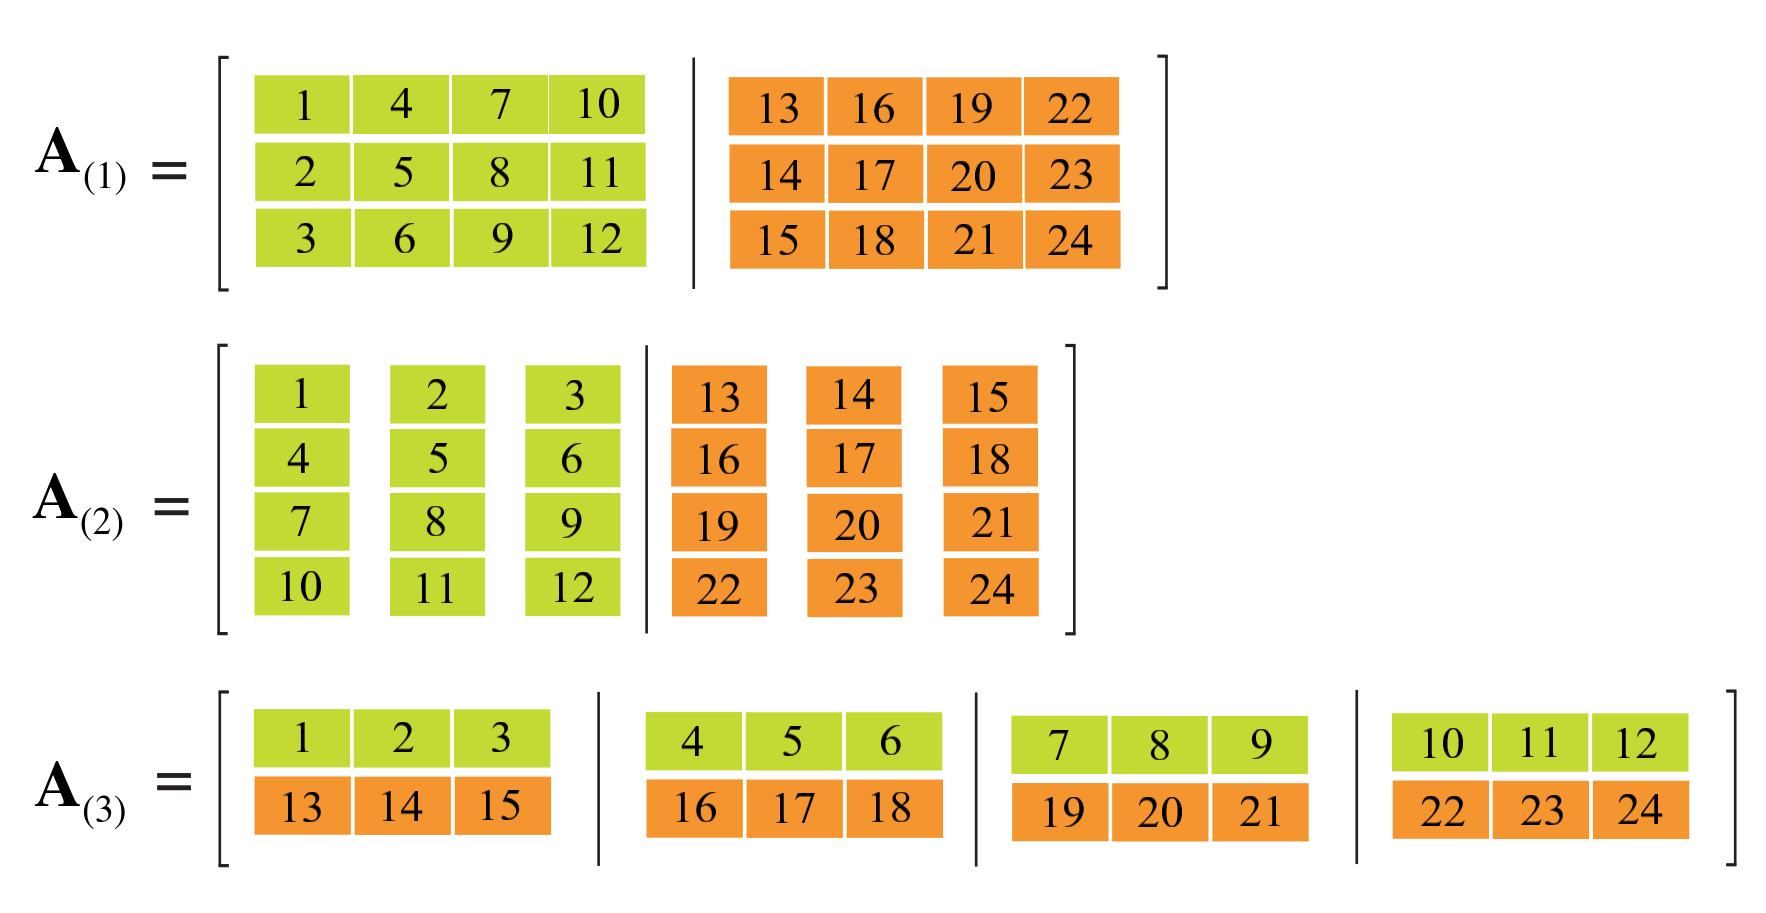
\includegraphics[width=\linewidth]{figs/tensor_unfolding2.png}
	\label{fig:tensor_unfolding2}
\end{figure}
\centering
$\mathbf{A}_{(i)}$ means mode-$i$ unfolding.
\end{columns}  %分栏环境结束

\end{frame}

\begin{frame}{Tensor Notations}
\begin{itemize}
\item Scalars are denoted by lowercase letters, e.g., $a$.
\item Vectors (tensors of order one) are denoted by boldface lowercase letters, e.g., $\mathbf{a}$.
\item Matrices (tensors of order two) are denoted by boldface capital letters, e.g., $\mathbf{A}$.
\item Higher-order tensors (order three or higher) are denoted by boldface Euler script letters, e.g., $\mathcal{X}$.
\item  The $n$-th element in a sequence is denoted by a superscript in parentheses, e.g., $\mathbf{A}^{(n)}$ denotes the $n$-th matrix in a sequence.
\item ``$\circ$'' represents the vector outer product.
\item $n$-mode product of a tensor $\mathcal{X}\in\mathbb{R}^{I_1 \times I_2 \times\cdots\times I_d}$ with a matrix $\mathbf{U}\in\mathbb{R}^{J\times I_n}$ is denoted by $\mathcal{X}\times_n \mathbf{U}$ and is of size $I_1 \times \cdots \times I_{n-1} \times J \times I_{n+1} \times \cdots \times I_d$,
$$
(\mathcal{X}\times_n\mathbf{U})_{i_1\cdots i_{n-1}ji_{n+1}\cdots i_d}=\sum_{i_n=1}^{I_n}x_{i_1i_2\cdots i_d}u_{ji_n}.
$$
\end{itemize}
\end{frame}

\begin{frame}{Tensor Notations}
\begin{itemize}
\item The Kronecker product of matrices $\mathbf{A}\in\mathbb{R}^{I\times J}$ and $\mathbf{A}\in\mathbb{R}^{K\times L}$ is denoted by $\mathbf{A} \otimes \mathbf{B}$.  The result is a matrix of size $(IK) \times (JL)$ and defined by
$$
\begin{aligned}
\mathbf{A} \otimes \mathbf{B} &= 
\left[\begin{matrix}
a_{11}\mathbf{B} & a_{12}\mathbf{B} & \cdots & a_{1J}\mathbf{B}\\
a_{21}\mathbf{B} & a_{22}\mathbf{B} & \cdots & a_{2J}\mathbf{B}\\
\vdots & \vdots & \ddots & \vdots\\
a_{I1}\mathbf{B} & a_{I2}\mathbf{B} & \cdots & a_{IJ}\mathbf{B}\\
\end{matrix}\right] \\
&=
\left[\begin{matrix}
\mathbf{a}_1\otimes\mathbf{b}_1 & \mathbf{a}_1\otimes\mathbf{b}_2 & \mathbf{a}_1\otimes\mathbf{b}_3 & \cdots & \mathbf{a}_J\otimes\mathbf{b}_{L-1} & \mathbf{a}_J\otimes\mathbf{b}_L
\end{matrix}\right].
\end{aligned}
$$
\item The Khatri-Rao product is the ``matching columnwise'' Kronecker product. Given matrices $\mathbf{A} \in \mathbb{R}^{I\times K}$ and $\mathbf{B} \in \mathbb{R}^{J\times K}$, their Khatri–Rao product is denoted by $\mathbf{A} \odot \mathbf{B}$. The result is a matrix of size $(IJ) \times K$ defined by
$$
\mathbf{A}\odot\mathbf{B}=
\left[\begin{matrix}
\mathbf{a}_1\otimes\mathbf{b}_1 & \mathbf{a}_2\otimes\mathbf{b}_2 & \cdots \mathbf{a}_K\otimes\mathbf{b}_K
\end{matrix}\right].
$$
\end{itemize}
\end{frame}

\begin{frame}{Agenda}
\begin{itemize}
    \large \item {Background}
    \large \item \textcolor{red}{Tensor Decompositions (CP, Tucker, and Tensor-Train/Tensor-Ring)}
    \large \item{Transform-based Tensor Model and Applications}
    \large \item{Tensor Computations (cuTensor, TensorDeC$++$)}
\end{itemize}
\end{frame}


\begin{frame}{Rank-One Tensor}
~~An $N$-way tensor $\mathcal{X}\in\mathbb{R}^{I_1\times I_2\times\cdots\times I_d}$ is \textit{rank one} if it can be written as the outer product of $d$ vectors:
$$
\mathcal{X}=\mathbf{a}^{(1)}\circ\mathbf{a}^{(2)}\circ\cdots\circ\mathbf{a}^{(d)}.
$$
%The symbol ``$\circ$'' represents the vector outer product. This means that each element 
%of the tensor is the product of the corresponding vector elements:
%$$
%x_{i_1i_2\cdots i_d}=a_{i_1}^{(1)}a_{i_2}^{(2)}\cdots a_{i_d}^{(d)}~~\text{for all}~1\leq i_n\leq I_n.
%$$
\textbf{example}. \textit{Rank-one} third-order tensor, $\mathcal{X} = a \circ b \circ c$. The $(i, j, k)$ element of $\mathcal{X}$ is given by $x_{ijk} = a_ib_jc_k$.
\begin{figure}
	\centering  
	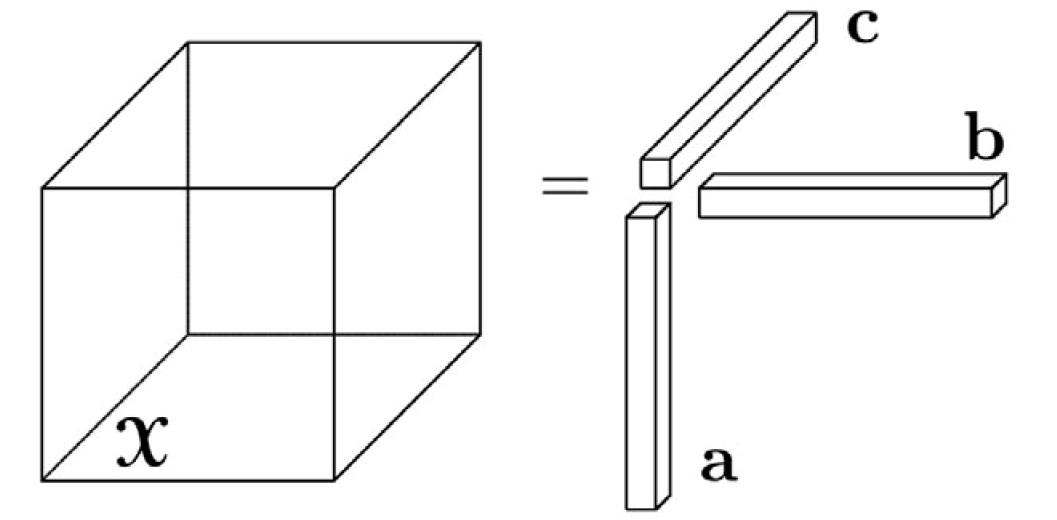
\includegraphics[width=0.45\linewidth]{figs/rankone_tensor.png}\\
	\label{fig:rankone_tensor}
\end{figure}
\end{frame}

\begin{frame}{CP Decomposition}
\vskip -1ex
\begin{figure}[t]
	\centering  
	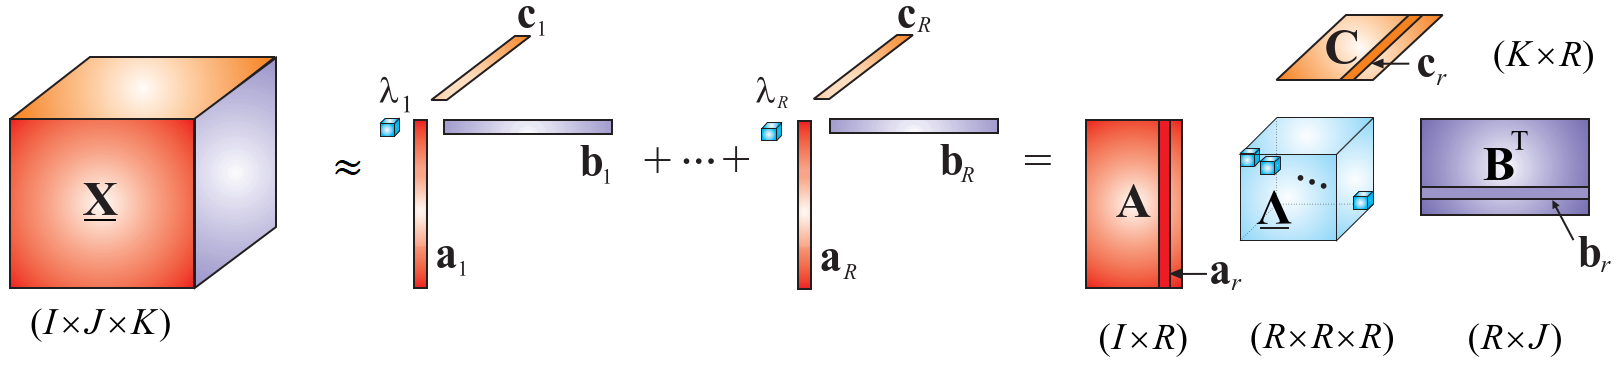
\includegraphics[width=\linewidth]{figs/cp_arch}
	\label{fig:cp_arch}
\end{figure}
\begin{columns}
\column{0.5\linewidth}
\vskip -6ex
\begin{mdframed}[backgroundcolor=brown!20,roundcorner=8pt,leftmargin=15pt,rightmargin=15pt]
\centering
\vskip -3ex
$$
\begin{aligned}
\mathcal{X}&\approx\sum_{r=1}^{R}\lambda_{r}\mathbf{a}_{r}\circ\mathbf{b}_{r}\circ\mathbf{c}_{r} \\
&=\mathbf{\Lambda}\times_{1}\mathbf{A}\times_{2}\mathbf{B}\times_{3}\mathbf{C} \\
&=[\![\mathbf{\Lambda};\mathbf{A},\mathbf{B},\mathbf{C}]\!]
\end{aligned}
$$
\end{mdframed}

\column{0.5\linewidth}
\vskip -8ex
\begin{align*}
\mathbf{X}_{(1)}&=\mathbf{A}\mathbf{\Lambda}(\mathbf{C}\odot\mathbf{B})^{T}+\mathbf{E}_{(1)} \\
\mathbf{X}_{(2)}&=\mathbf{B}\mathbf{\Lambda}(\mathbf{C}\odot\mathbf{A})^{T}+\mathbf{E}_{(2)} \\
\mathbf{X}_{(3)}&=\mathbf{C}\mathbf{\Lambda}(\mathbf{B}\odot\mathbf{A})^{T}+\mathbf{E}_{(3)}
\end{align*}

\end{columns}
\end{frame}


\begin{frame}{CP Decomposition}
\large
\begin{table}
\begin{tabular}{l | l}
\textbf{Name} & \textbf{Proposed by} \\
\hline \hline
Polyadic form of a tensor & Hitchcock, 1927 \\ 
PARAFAC (parallel factors) & Harshman, 1970\\
CANDECOMP or CAND (canonical decomposition) & Carroll and Chang, 1970\\
Topographic components model & Mocks, 1988 \\
CP (CANDECOMP/PARAFAC) & Kiers, 2000
\end{tabular}
\caption{Some of the many names for the CP decomposition.}
\end{table}
\end{frame}

\begin{frame}{Tucker Decomposition}
\vskip -2ex
\begin{figure}[t]
	\centering  
	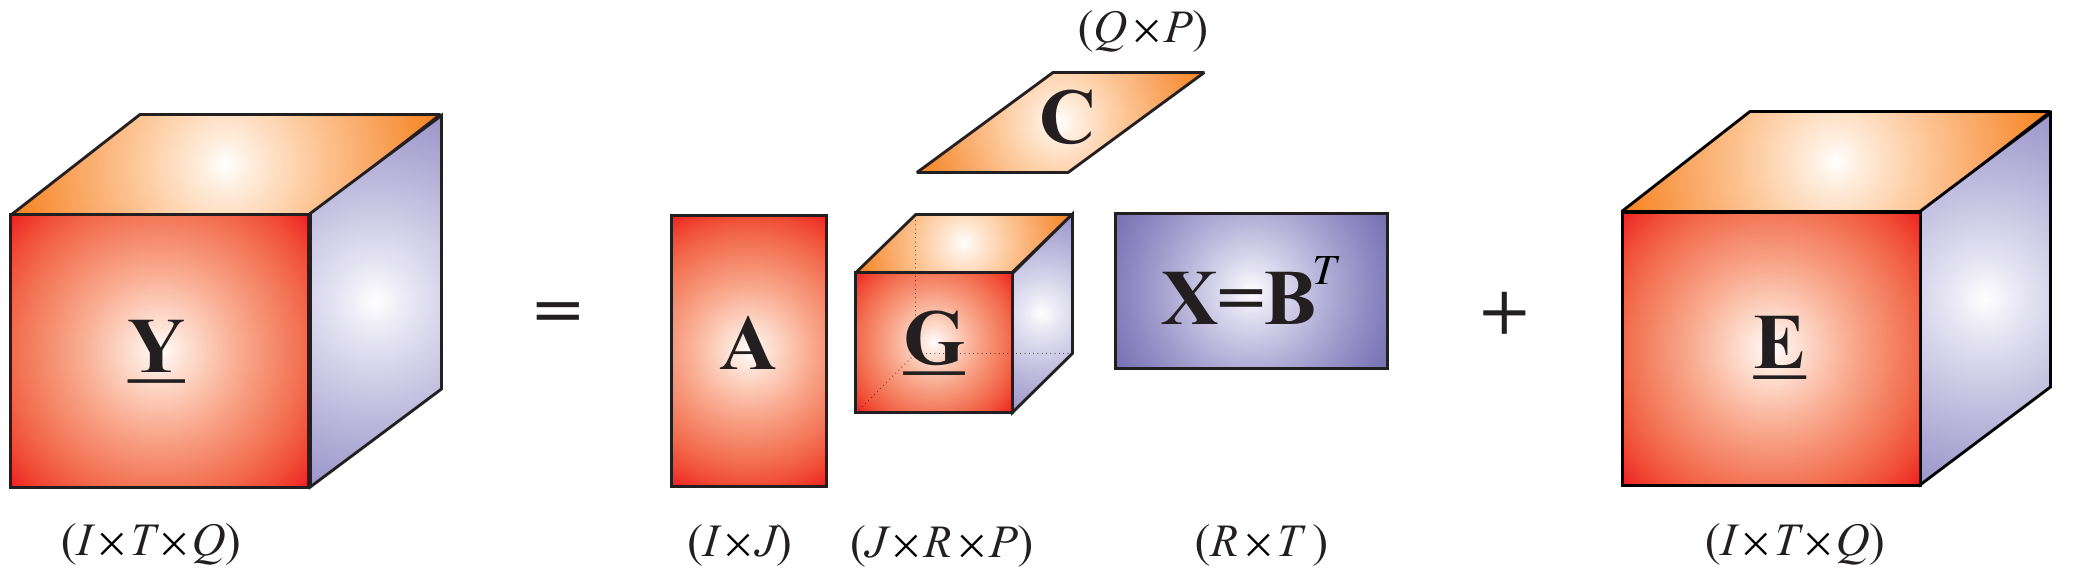
\includegraphics[width=0.95\linewidth]{figs/tucker_arch}
	\label{fig:tucker_arch}
\end{figure}
\vskip -2.5ex
\begin{mdframed}[backgroundcolor=brown!20,roundcorner=8pt,leftmargin=60pt,rightmargin=60pt]
\centering
$
\mathcal{Y}=\mathcal{G}\times_{1}\mathbf{A}\times_{2}\mathbf{B}\times_{3}\mathbf{C}+\mathcal{E}=[\![\mathcal{G};\mathbf{A},\mathbf{B},\mathbf{C}]\!]+\mathcal{E}
$
\end{mdframed}
\vskip -0.5ex
\begin{align*}
\mathbf{X}_{(1)}&\approx\mathbf{A}\mathbf{G}_{(1)}(\mathbf{C}\otimes\mathbf{B})^{T}\\
\mathbf{X}_{(2)}&\approx\mathbf{B}\mathbf{G}_{(2)}(\mathbf{C}\otimes\mathbf{A})^{T}\\
\mathbf{X}_{(3)}&\approx\mathbf{C}\mathbf{G}_{(3)}(\mathbf{B}\otimes\mathbf{A})^{T}
\end{align*}
\end{frame}

\begin{frame}{Tucker Decomposition}
\large
\begin{table}
\begin{tabular}{l | l}
Name & Proposed by \\
\hline \hline
Three-mode factor analysis (3MFA/Tucker3) & Tucker, 1966 \\ 
Three-mode PCA (3MPCA) &  Kroonenberg and De Leeuw, 1980\\
N-mode PCA & Kapteyn et al., 1986 \\
Higher-order SVD (HOSVD)  & De Lathauwer et al., 2000 \\
N-mode SVD & Vasilescu and Terzopoulos, 2002
\end{tabular}
\caption{Names for the Tucker decomposition (some specific to three-way and some for N-way).}
\end{table}
\end{frame}

%\begin{frame}{Tensor Train Decomposition}
%\large
%\begin{block}{Low-rank Decomposition}
%$$
%\begin{aligned}
%&\mathbf{A}=\mathbf{G}_{1}\mathbf{G}_{2}  \\
%&\mathbf{G}_{1}\text{: collection of rows, }\mathbf{G}_{2}\text{: collection of columbs}\\
%&\mathbf{A}_{i_1i_2}=\underbrace{\mathbf{G}_1(i_1)}_{1\times R}\underbrace{\mathbf{G}_2(i_2)}_{R\times 1}
%\end{aligned}
%$$
%\end{block}
%\begin{figure}
%	\centering  
%	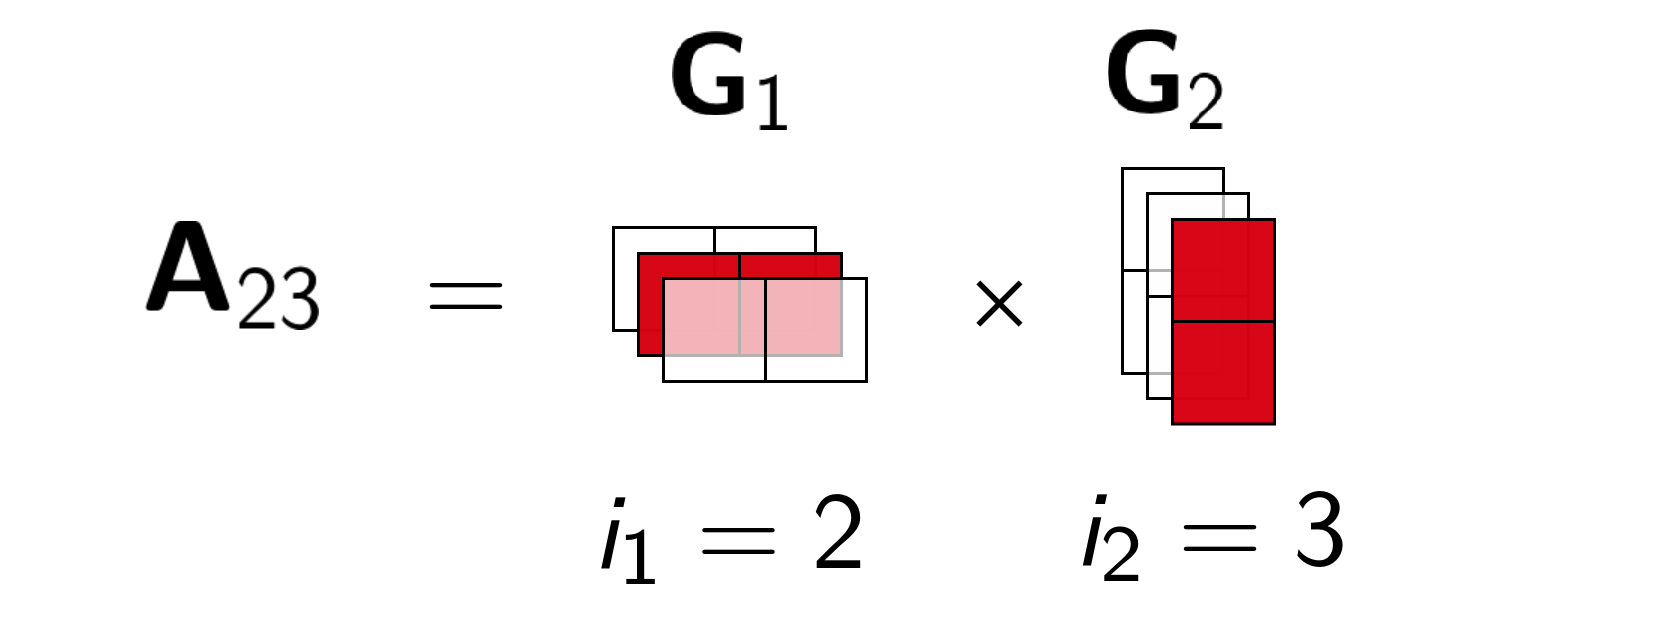
\includegraphics[width=0.45\linewidth]{figs/tt_lowrank.png}
%	\label{fig:tt_lowrank}
%\end{figure}
%\end{frame}

\begin{frame}{Tensor Train Decomposition}
\large
\begin{block}{TT Form}
$$
\mathcal{A}_{i_1i_2\cdots i_d}=\underbrace{\mathcal{G}_{1}(i_1)}_{1\times R}\underbrace{\mathcal{G}_{2}(i_2)}_{R\times R}\cdots\underbrace{\mathcal{G}_{d}(i_d)}_{R\times 1}
$$
\end{block}
\normalsize
\begin{figure}
	\centering  
	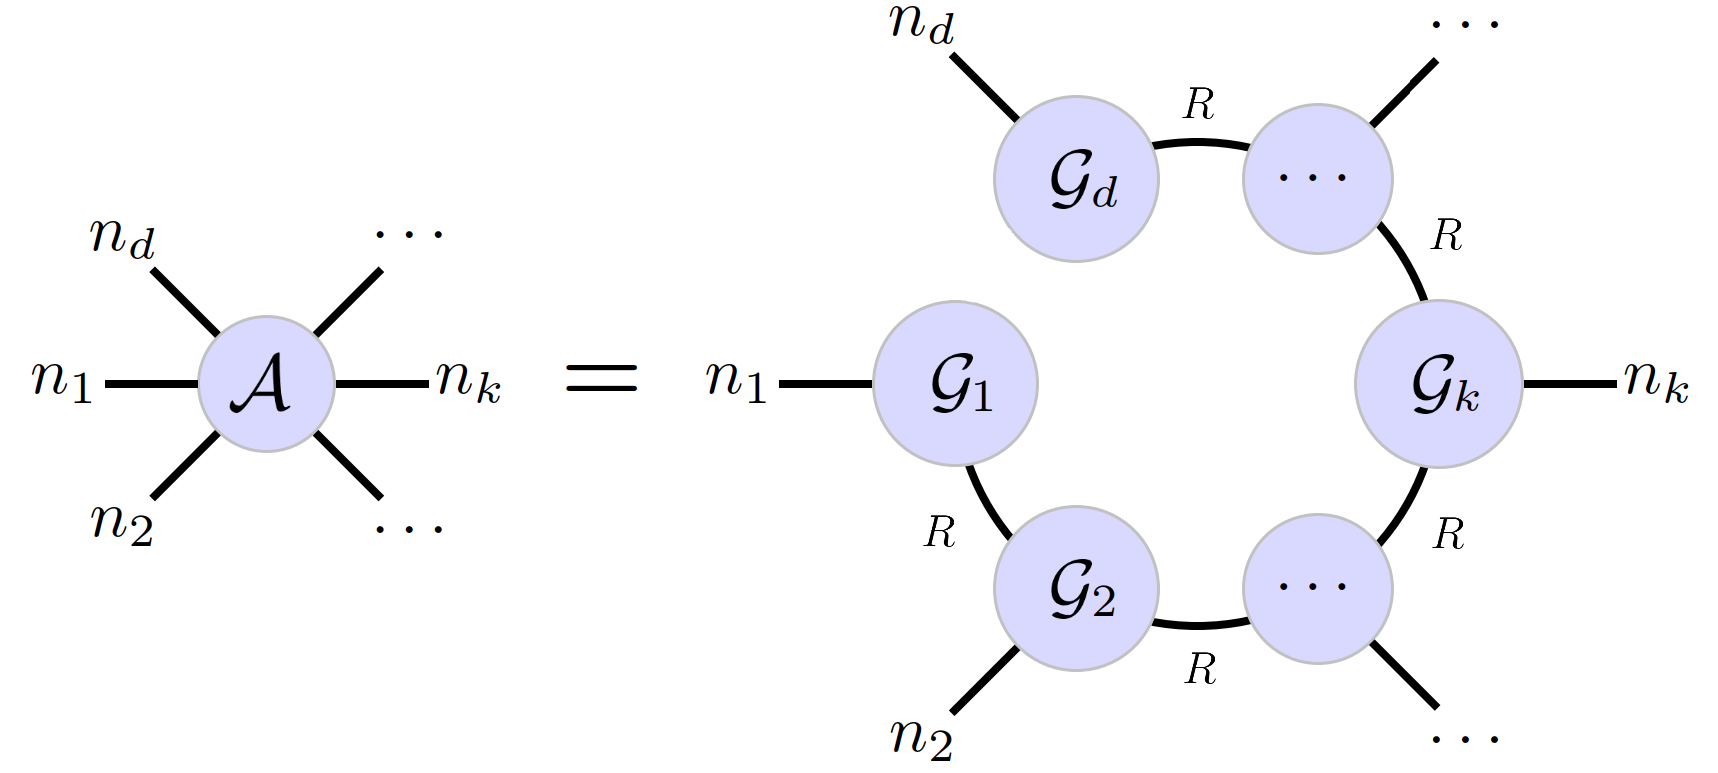
\includegraphics[width=0.45\linewidth]{figs/tensor_train_arch.png} \\
	A graphical representation of the tensor train decomposition
	\label{fig:tensor_train_arch}
\end{figure}
\end{frame}

\begin{frame}{Tensor Ring Decomposition}
\textbf{Example}.
\begin{figure}
	\centering  
	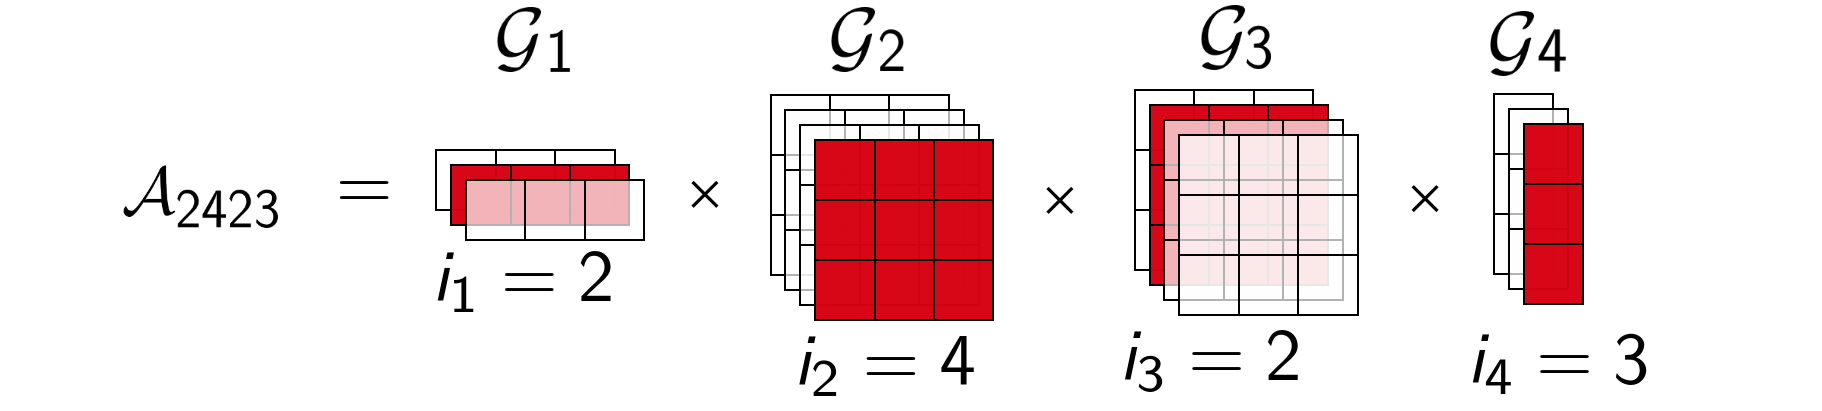
\includegraphics[width=\linewidth]{figs/tt_form_example.png}
	\label{fig:tt_form_example}
\end{figure}
\end{frame}

\begin{frame}{Tensor Ring Decomposition}
\large
\begin{block}{TR Form}
$$
\begin{aligned}
\mathcal{A}_{i_1i_2\cdots i_d}=\text{Tr}\{\mathcal{Z}_1(i_1)\mathcal{Z}_2(i_2)\cdots\mathcal{Z}_d(i_d)\}
=\text{Tr}\left\{\prod_{k=1}^{d}\mathcal{Z}_k(i_k)\right\}
\end{aligned}
$$
\end{block}
\normalsize
\begin{figure}
	\centering  
	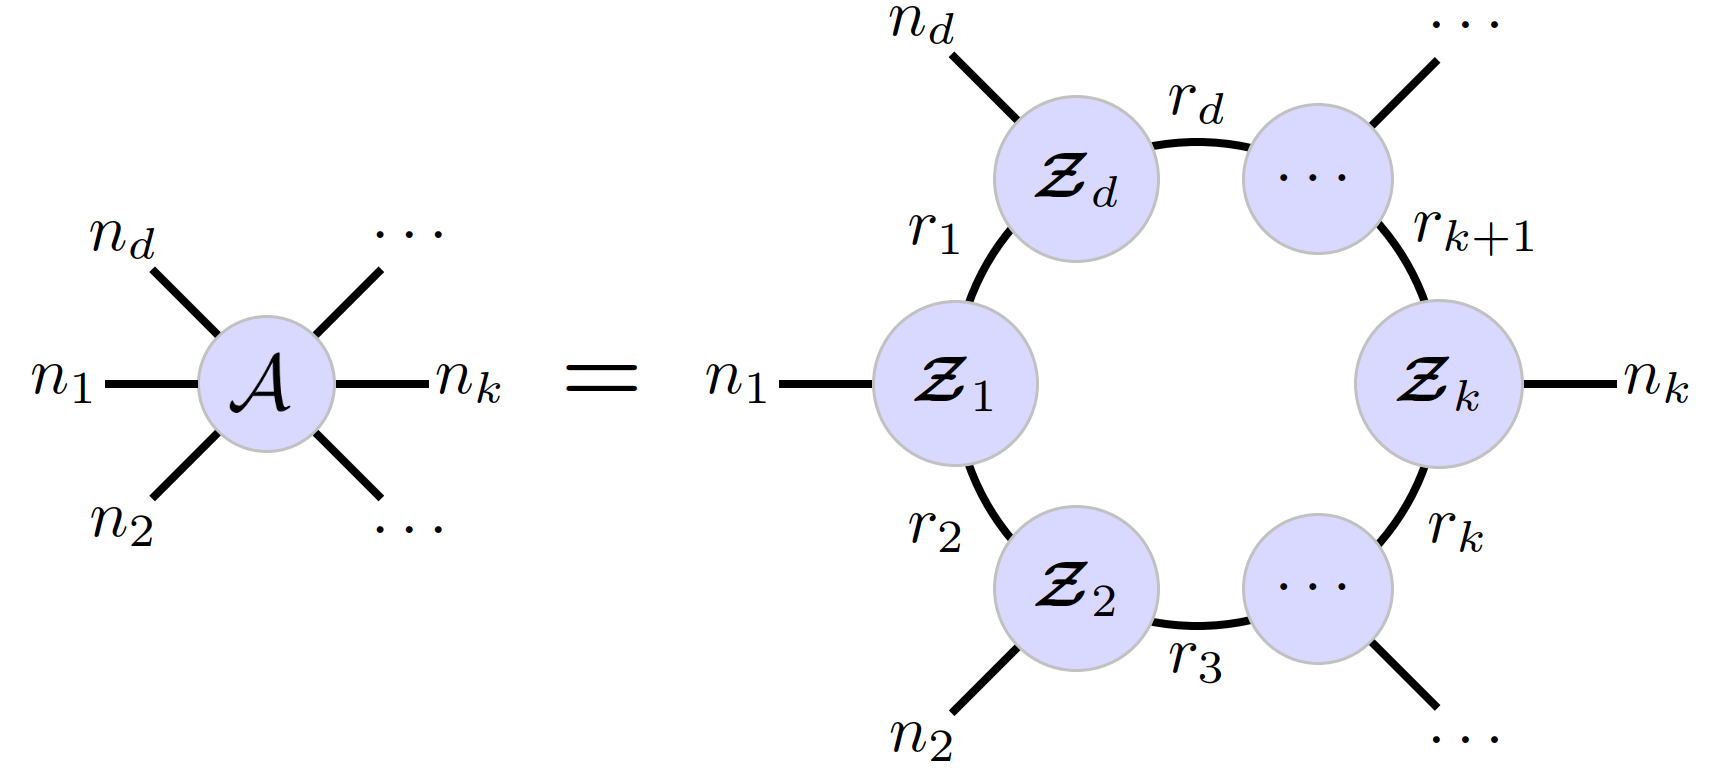
\includegraphics[width=0.45\linewidth]{figs/tensor_ring_arch.png} \\
	A graphical representation of the tensor ring decomposition
	\label{fig:tensor_ring_arch}
\end{figure}
\end{frame}

\begin{frame}{Agenda}
\begin{itemize}
    \large \item {Background}
    \large \item {Tensor Decompositions (CP, Tucker, and Tensor-Train/Tensor-Ring)}
    \large \item \textcolor{red}{Transform-based Tensor Model and Applications}
    \large \item{Tensor Computations (cuTensor, TensorDeC$++$)}
\end{itemize}
\end{frame}


\begin{frame}{Transform-based Model}
\begin{block}{Basic Operators}
~~The operator $\texttt{matview}(\cdot)$ takes a tensor $\mathcal{A}\in\mathbb{C}^{n_1\times n_2\times n_3\times n_4}$ and returns an $n_1n_3n_4\times n_2n_3n_4$ block diagonal matrix, with each block being an $n_1\times n_2$ matrix, defined as
$$
\texttt{matview}(\mathcal{A})=\text{diag}(\mathbf{A}^1, \cdots, \mathbf{A}^p, \cdots, \mathbf{A}^P), ~ p\in [P], 
$$
and
$$
\mathbf{A}^p(i,j)=\mathcal{A}(i,j,k,l), ~p=(l-1)n_3+k, i\in[n_1], ~j\in[n_2], ~k\in [n_3], ~l\in[n_4],
$$
where $P=n_3n_4$, and $[n]$ denotes the index set $\{1, 2, \cdots, n\}$. The operator $\texttt{tenview}(\cdot)$ folds $\texttt{matview}(\mathcal{A})$ back to tensor $\mathcal{A}$, i.e.,
$$
\texttt{tenview}(\texttt{matview}(\mathcal{A})) = \mathcal{A}.
$$
\end{block}
\end{frame}

\begin{frame}{Transform-based Model}
\begin{block}{Basic Operators}
~~Given two fourth-order tensors $\mathcal{A}\in\mathbb{C}^{n_1\times n' \times n_3 \times n_4}$ and $\mathcal{B}\in\mathbb{C}^{n' \times n_2 \times n_3 \times n_4}$, the corresponding $p$-th matrices are $\mathbf{A}^{p} \in \mathbb{C}^{n_1\times n'}$ and $\mathbf{B}^{p} \in \mathbb{C}^{n' \times n_2}$, and their multiplication is well-defined as $\mathbf{C}^p = \mathbf{A}^p\mathbf{B}^p \in \mathbb{C}^{n_1\times n_2}$. Later in the transform domain, we will need the following matrix multiplication of two block diagonal matrices, e.g.,
$$
\texttt{matview}(\mathcal{C})=\texttt{matview}(\mathcal{A})\cdot\texttt{matview}(\mathcal{B}),
$$
where $\cdot$ denotes the conventional matrix multiplication.
\end{block}
\end{frame}

\begin{frame}{Transform-based Model}
\vskip -1ex
\begin{block}{Tensor-scalar multiplication}
~~Given an invertible 2D discrete transform $\mathcal{L}:\mathbb{C}^{1\times 1\times n_3\times n_4} \to \mathbb{C}^{1\times 1\times n_3\times n_4}$, the element-wise multiplication $\circ$, and $\alpha, \beta \in \mathbb{C}^{1\times 1\times n_3\times n_4}$, we define the tensor-scalar multiplication
$$
\alpha\bullet\beta\triangleq\mathcal{L}^{-1}(\mathcal{L}(\alpha)\circ\mathcal{L}(\beta)),
$$
where $\mathcal{L}^{-1}:\mathbb{C}^{1\times 1\times n_3\times n_4} \to \mathbb{C}^{1\times 1\times n_3\times n_4}$ is the inverse transform.
\end{block}
\begin{block}{Tensor-linear combinations}
~~Given tensor scalars $c_j \in\mathbb{C}^{1\times 1\times n_3\times n_4}, j\in[n_2]$, a tensor-linear combination of the tensor-columns $\mathcal{A}_j \in \mathbb{C}^{n_1\times 1\times n_3\times n_4}, j\in[n_2]$, is defined as
$$
\mathcal{A}_1\bullet c_1 + \cdots + \mathcal{A}_{n_2}\bullet c_{n_2}=\mathcal{A}\bullet\mathbf{c},
$$
where $\mathcal{A}=[\mathcal{A}_1, \cdots, \mathcal{A}_{n_2}]$ and $\mathbf{c}=[c_1, \cdots, c_{n_2}]^T$.

\end{block}
\end{frame}

\begin{frame}{Transform-based Model}
\begin{block}{$\mathcal{L}$-product}
~~The $\mathcal{L}$-product $\mathcal{C}=\mathcal{A}\bullet\mathcal{B}\in\mathbb{C}^{n_1\times n_2\times n_3\times n_4}$ of $\mathcal{A}\in \mathbb{C}^{n_1\times n'\times n_3\times n_4}$ and $\mathcal{B}\in\mathbb{C}^{n'\times n_2\times n_3\times n_4}$ is defined as
$$
\mathcal{C}(i,j)=\sum_{k\in[n']}\mathcal{A}(i,k)\bullet\mathcal{B}(k,j), ~i\in[n_1], ~j\in[n_2].
$$
\end{block}
\textbf{Lemma}. The $\mathcal{L}$-product $\mathcal{C}=\mathcal{A}\bullet\mathcal{B}$ can be calculated in the following way: First, we compute
$$
\texttt{matview}(\widetilde{\mathcal{C}})=\texttt{matview}(\widetilde{\mathcal{A}})\cdot\texttt{matview}(\widetilde{\mathcal{B}}).
$$
Then, we stack $\texttt{matview}(\widetilde{\mathcal{C}})$ back to tensor $\texttt{tenview}(\texttt{matview}(\widetilde{\mathcal{C}}))$ and perform the inverse transform to get $\mathcal{C}$, i.e., $\mathcal{C}=\mathcal{L}^{-1}(\widetilde{\mathcal{C}})$. The notation $\widetilde{\mathcal{A}}$ denotes the transform-domain representation of $\mathcal{A}\in\mathbb{C}^{n_1\times n_2\times n_3\times n_4}$ such that $\widetilde{\mathcal{A}}=\mathcal{L}(\mathcal{A})$ and $\mathcal{A}=\mathcal{L}^{-1}(\widetilde{\mathcal{A}})$.

\end{frame}

\begin{frame}{Transform-based Model}
So the $\mathcal{L}$-product can be considered as
$$
\mathcal{L}(\mathcal{C}(i,j))=\sum_{k\in[n']}\mathcal{L}(\mathcal{A}(i,k))\circ\mathcal{L}(\mathcal{B}(k,j)),
$$
which can be represented as $\widetilde{\mathbf{C}^p}=\widetilde{\mathbf{A}^p}\widetilde{\mathbf{B}^p}, ~p\in[P]$.
\end{frame}

\begin{frame}{Low-tubal-rank Model}
\vskip -1ex
\begin{block}{Notations}
$$\vec{\mathcal{A}}_i\equiv\mathcal{A}(:,i,:),~~~~\mathbf{A}^{(j)}\equiv\mathcal{A}(:,:,j),~~~~\hat{\mathcal{A}} := \texttt{fft}(\mathcal{A}, [], 3)$$
\vskip -1ex
$$
\texttt{bcirc}(\mathcal{A})=\left[
  \begin{matrix}
   \mathbf{A}^{(1)} & \mathbf{A}^{(n)} & \mathbf{A}^{(n-1)} & \cdots & \mathbf{A}^{(2)} \\
   \mathbf{A}^{(2)} & \mathbf{A}^{(1)} & \mathbf{A}^{(n)} & \cdots & \mathbf{A}^{(3)} \\
   \vdots & \vdots & \vdots & \ddots & \vdots \\
    \mathbf{A}^{(n)} & \mathbf{A}^{(n-1)} & \cdots & \mathbf{A}^{(2)} & \mathbf{A}^{(1)}
  \end{matrix}
  \right]
$$
$$
\texttt{unfold}(\mathcal{A})=\left[
  \begin{matrix}
    \mathbf{A}^{(1)} \\
    \mathbf{A}^{(2)} \\
    \vdots \\
    \mathbf{A}^{(n)}
  \end{matrix}
\right], ~~~~~~~~\texttt{fold}(\texttt{unfold}(\mathcal{A}))=\mathcal{A}
$$
\end{block}
\end{frame}



\begin{frame}{Low-tubal-rank Model}
\begin{block}{t-Product}
$$\mathcal{A}*\mathcal{B}=\texttt{fold}(\texttt{bcirc}(\mathcal{A})\cdot\texttt{unfold}(\mathcal{B}))$$
\end{block}
\textbf{Example}. Let $\mathcal{A}\in\mathbb{R}^{3\times 2 \times 2}$ with frontal faces
$$
%\renewcommand\arraystretch{1.3}
\mathbf{A}^{(1)}=\left[
\begin{array}{c c}
  1 & 0 \\
  0 & 2 \\
  -1 & 3
\end{array}
\right]~~~~
\text{and}~~~~\mathbf{A}^{(2)}=\mleft[
\begin{array}{c c}
  -2 & 1 \\
  -2 & 7 \\
  0 & -1
\end{array}
\mright],
$$
and let $\vec{\mathcal{B}}\in\mathbb{R}^{2\times 1 \times 2}$ with frontal faces
$$
\mathbf{B}^{(1)}=
\left[\begin{matrix}
3\\
-1
\end{matrix}\right]
~~~~\text{and}~~~~
\mathbf{B}^{(2)}=
\left[\begin{matrix}
-2\\
-3
\end{matrix}\right].
$$
\end{frame}

\begin{frame}{Low-tubal-rank Model}
$$
\begin{aligned}
\mathcal{A}*\vec{\mathcal{B}} & =\texttt{fold}\left(
\left[\begin{array}{cc|cc}
1 & 0 & -2 & 1\\
0 & 2 & -2 & 7\\
-1 & 3 & 0 & -1\\
\hline
-2 & 1 & 1 & 0\\
-2 & 7 & 0 & 2\\
0 & -1 & -1 & 3
\end{array}\right]
\left[\begin{array}{c}
3\\
-1\\
\hline
-2\\
-3
\end{array}\right]
\right)\\
& = \texttt{fold}\left(
\left[\begin{array}{c}
4\\
-19\\
-3\\
\hline
-9\\
-19\\
-6
\end{array}\right]
\right)\in\mathbb{R}^{3\times 1 \times 2}
\end{aligned}
$$
is a $3 \times 1 \times 2$ tensor. In other words, in this example, $\vec{\mathcal{C}} := \mathcal{A} * \vec{\mathcal{B}}$ is a $3\times 2$ matrix, oriented as a lateral slice of a third-order tensor.
\end{frame}

\begin{frame}{Low-tubal-rank Model}
\begin{block}{t-Linear combinations}
~~~~Given $k$ tubal scalars $\vec{\mathbf{c}}_j\in\mathbb{R}^{1\times 1\times n},~j=1,2,\cdots,k$, a t-linear combination of $\vec{\mathcal{X}}_j\in \mathbb{R}^{m\times 1\times n},~j=1,2,\cdots,k$ is defined as
$$
\vec{\mathcal{X}}_1*\vec{\mathbf{c}}_1 + \vec{\mathcal{X}}_2 * \vec{\mathbf{c}}_2 + \cdots + \vec{\mathcal{X}}_k * \vec{\mathbf{c}}_k \equiv \mathcal{X} * \vec{\mathcal{C}}
$$
where
$$
\mathcal{X} := \left[\vec{\mathcal{X}}_1, \vec{\mathcal{X}}_2, \cdots, \vec{\mathcal{X}}_k\right],~~~~\vec{\mathcal{C}}:=\left[\begin{matrix}
\vec{\mathbf{c}}_1\\
\vec{\mathbf{c}}_2\\
\vdots\\
\vec{\mathbf{c}}_k
\end{matrix}\right].
$$
\end{block}
\textbf{Example}. Using $\mathcal{A}\in\mathbb{R}^{3\times 2 \times 2}$ and $\vec{\mathcal{B}}\in\mathbb{R}^{2\times 1\times 2}$ from the previous example, we see that

\end{frame}

\begin{frame}{Low-tubal-rank Model}
$$
\begin{aligned}
\mathcal{A}*\vec{\mathcal{B}} & = \vec{\mathcal{A}}_1 * \vec{\mathbf{b}}_{11} + \vec{\mathcal{A}}_2 * \vec{\mathbf{b}}_{21} \\
& = \texttt{fold}\left(
\left[\begin{array}{c}
7\\
4\\
-3\\
\hline
-8\\
-6\\
2
\end{array}\right]
\right) + \texttt{fold}\left(
\left[\begin{array}{c}
-3\\
-23\\
0\\
\hline
-1\\
-13\\
-8
\end{array}\right]
\right)=\texttt{fold}\left(
\left[\begin{array}{c}
4\\
-19\\
-3\\
\hline
-9\\
-19\\
-6
\end{array}\right]
\right)
\end{aligned}
$$
Thus, $\vec{\mathcal{C}} := \mathcal{A} * \vec{\mathcal{B}}$ is a t-linear combination of the lateral slices of $\mathcal{A}$.
\end{frame}

\begin{frame}{Low-tubal-rank Model}

\begin{block}{Observation}
~~~~Given $\vec{\mathbf{a}}, \vec{\mathbf{b}} \in \mathbb{R}^{1\times 1\times n}$, $\vec{\mathbf{a}} * \vec{\mathbf{b}}$ can be computed as
$$
\vec{\mathbf{a}} * \vec{\mathbf{b}} := \texttt{ifft}(\hat{\vec{\mathbf{a}}} \circledcirc \hat{\vec{\mathbf{b}}}, [], 3),
$$
where $\circledcirc$ of two tubal scalars means pointwise multiplication.\\
~~~~Factorizations of $\mathcal{A}$ are created (implicitly) by applying the appropriate matrix factorization to each of the $\hat{\mathcal{A}}^{(i)}$
$$
\mathcal{A}=\mathcal{Q} * \mathcal{R} \Longleftrightarrow \hat{\mathcal{A}}^{(i)}=\hat{\mathcal{Q}}^{(i)}\hat{\mathcal{R}}^{(i)}.
$$
\end{block}
\end{frame}

\begin{frame}{Low-tubal-rank Model}
\begin{block}{t-SVD}
$$
\mathcal{A}=\mathcal{U}*\mathcal{S}*\mathcal{V}^{T}=\sum_{i=1}^{\text{min}(l,m)}\vec{\mathcal{U}}_i*\mathbf{s}_i*\vec{\mathcal{V}}_i^T, ~~~~\mathbf{s}_i :=\mathcal{S}(i,i,:)
$$
\end{block}
\vskip -2ex
\begin{figure}
	\centering  
	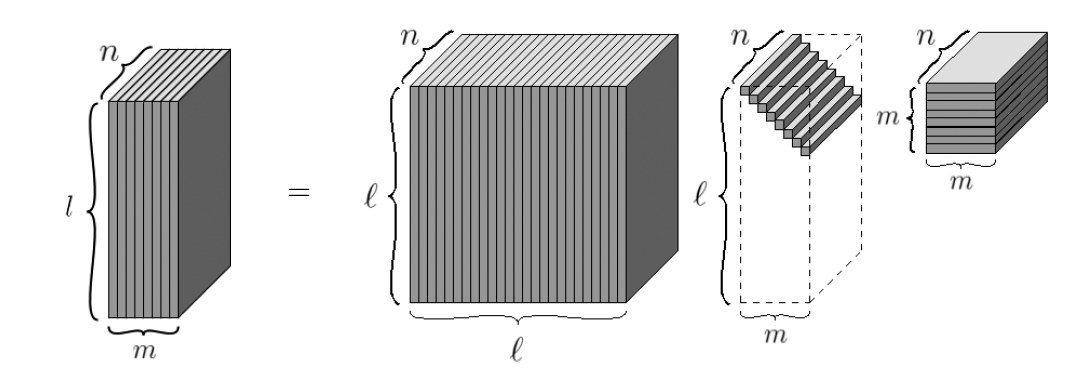
\includegraphics[width=0.7\linewidth]{figs/tsvd_arch.png}\\
	The t-SVD of an $l \times m \times n$ tensor
	\label{fig:tsvd_arch}
\end{figure}
\end{frame}

\begin{frame}{Tubal-tensor Sparse Coding}
\begin{block}{Tubal-tensor Linear Combination}
A two-dimensional image of size $m \times k$ is represented by a third-order tensor $\mathcal{X}\in \mathbb{R}^{m\times 1 \times k}$, which can be approximated by the t-product between $\mathcal{D}\in\mathbb{R}^{m\times r\times k}$ and $\mathcal{C}\in\mathbb{R}^{r\times 1 \times k}$ as
$$
\begin{aligned}
\mathcal{X} & = \mathcal{D} * \mathcal{C}\\
& = \mathcal{D}(:,1,:)*\mathcal{C}(1,1,:) + \mathcal{D}(:,2,:)*\mathcal{C}(2,1,:) + \cdots + \mathcal{D}(:,r,:)*\mathcal{C}(r,1,:)
\end{aligned}
$$
\end{block}
\vskip -2ex
\begin{figure}
	\centering  
	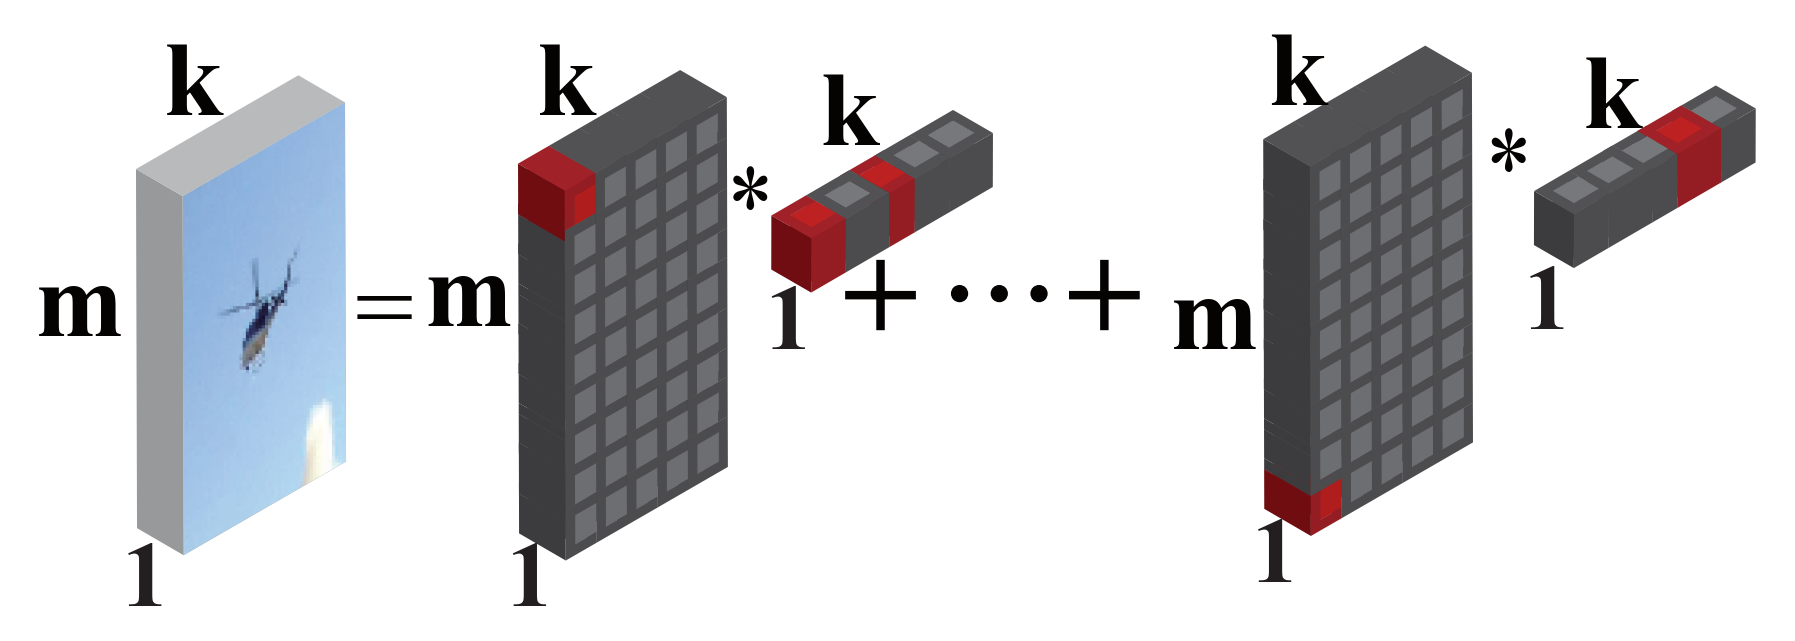
\includegraphics[width=0.5\linewidth]{figs/tubaltensor_arch.png}\\
	Tubal-tensor sparse coding model is based on circular convolution operation
	\label{fig:tubaltensor_arch}
\end{figure}

\end{frame}

\begin{frame}{Tubal-tensor Sparse Coding}
\begin{block}{Tubal-tensor Sparse Representation}
~~~~A third-order tensor $\mathcal{X} \in \mathbb{R}^{m\times n\times k}$ is presented by $n$ images of size $m \times k$. Let $\mathcal{D} \in \mathbb{R}^{m\times r\times k}$ be the tensor dictionary, where each lateral slice $\mathcal{D}(:,j,:)$ represents a tensor basis, and $\mathcal{C}\in \mathbb{R}^{r\times n \times k}$ be the tensor corresponding representations. Each image $\mathcal{X}(:,j,:)$ is approximated by a sparse t-linear combination of those tensor bases. Tubal-tensor sparse coding (TubSC) model can be formulated as
$$
\begin{aligned}
\min_{\mathcal{D},\mathcal{C}}&~~~\frac{1}{2}\|\mathcal{X}-\mathcal{D}*\mathcal{C}\|_{F}^{2}+\beta\|\mathcal{C}\|_1 \\
\text{s.t.} &~~~ \|\mathcal{D}(:,j,:)\|_F^2\le 1, j=1,2,\cdots,r.
\end{aligned}
$$
\end{block}
~~~~~TubSC model can be solved alternately by \textbf{tensor coefficients learning} and \textbf{tensor dictionary learning}.
\end{frame}

\begin{frame}{Tubal-tensor Sparse Coding}
\begin{block}{Tensor Coefficients Learning}
$$
\min_{\mathcal{C}}~~\frac{1}{2}\|\mathcal{X}-\mathcal{D}*\mathcal{C}\|_F^2+\beta\|\mathcal{C}\|_1
$$
~~~~According to low-tubal-tensor model, the problem can be transformed to
$$
\min_{\texttt{unfold}(\mathcal{C})}~~\frac{1}{2}\|\texttt{unfold}(\mathcal{X})-\texttt{bcirc}(\mathcal{D})\cdot\texttt{unfold}(\mathcal{C})\|_F^2+\beta\|\texttt{unfold}(\mathcal{C})\|_1.
$$
It can be solved by Iterative Shrinkage Thresholding algorithm based on Tensor (\textbf{ISTT}), which is rewritten as
$$
\min_{\mathcal{C}}~~f(\mathcal{C})+\beta g(\mathcal{C}),
$$
where $f(\mathcal{C}) = \frac{1}{2}\|\mathcal{X}-\mathcal{D}*\mathcal{C}\|_F^2,~\text{and}~g(\mathcal{C}) = \|\mathcal{C}\|_1$.
\end{block}
\end{frame}

\begin{frame}{Tubal-tensor Sparse Coding}
\begin{block}{Tensor Dictionary Learning}
\vskip -1ex
$$
\begin{aligned}
\min_{\mathcal{D}}&~~~\frac{1}{2}\|\mathcal{X}-\mathcal{D}*\mathcal{C}\|_{F}^{2}\\
\text{s.t.} &~~~ \|\mathcal{D}(:,j,:)\|_F^2\le 1, j=1,2,\cdots,r.
\end{aligned}
$$
~~~~We transform this problem into the frequecy domain:
\vskip -1ex
$$
\begin{aligned}
\min_{\hat{\mathcal{D}}^{(l)}}&~~~\sum_{l=1}^{k}\|\hat{\mathcal{X}}^{(l)}-\hat{\mathcal{D}}^{(l)}\hat{\mathcal{C}}^{(l)}\|_F^2,l=1,2,\cdots,k\\
\text{s.t.}&~~~\sum_{l=1}^{k}\|\hat{\mathcal{D}}^{(l)}(:,j)\|_F^2\le k, j=1,2,\cdots,r.
\end{aligned}
$$
~~~~Then adopt the Lagrange dual (Lee et al. 2007) to solve the dual variables by Newton’s algorithm.
\end{block}
\end{frame}

\begin{frame}{Agenda}
\begin{itemize}
    \large \item {Background}
    \large \item {Tensor Decompositions (CP, Tucker, and Tensor-Train/Tensor-Ring)}
    \large \item {Transform-based Tensor Model and Applications}
    \large \item \textcolor{red}{Tensor Computations (cuTensor, TensorDeC$++$)}
\end{itemize}
\end{frame}

\begin{frame}{cuTensor-tubal (GPU)}

\begin{columns}
\column{0.57\linewidth}
This library is a general approach to compute low-tubal-rank tensor operations in the frequency domain on GPUs.
\begin{enumerate}
  \item Obtain the frequency domain representation of the input tensor by performing Fourier transform along the third dimension (called tube-wise DFT) on the GPU;
  \item In the frequency domain, the tensor operations are separated into multiple independent complex matrix computations that possess strong parallelism;
  \item Converting the frequency domain results back to the time domain through inverse Fourier transform along the third dimension on the GPU (called tube-wise inverse DFT).
\end{enumerate}
\column{0.45\linewidth}
\begin{figure}
	\centering  
	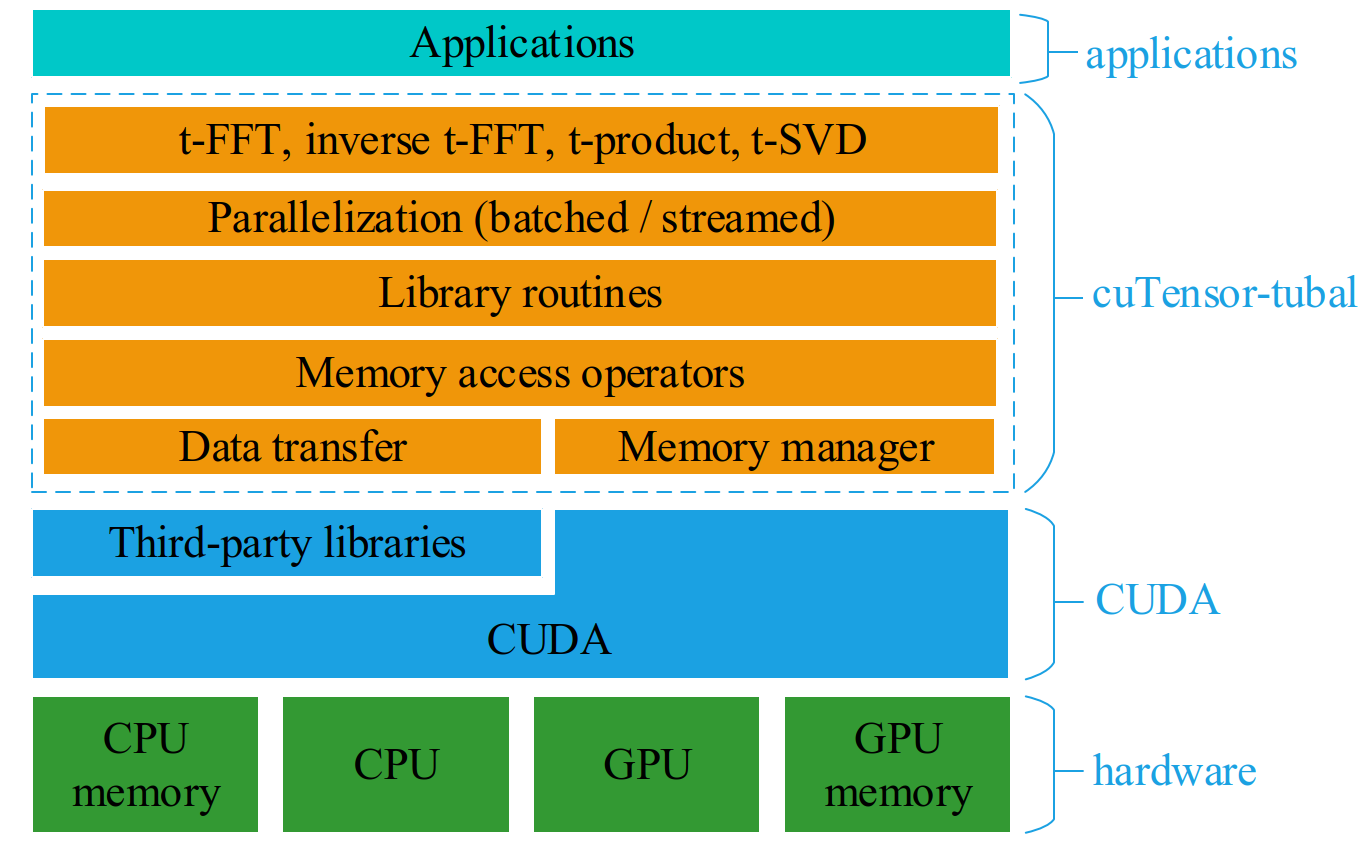
\includegraphics[width=\linewidth]{figs/cutensor_arch.png}\\
	System architecture of the cuTensor-tubal library
	\label{fig:cutensor_arch}
\end{figure}
\end{columns}
\end{frame}

\begin{frame}{cuTensor-tubal (GPU)}

\begin{table}
$\begin{array}{l | l | l}
\textbf{Operation} & \textbf{Input} & \textbf{Output} \\
\hline \hline
\text{t-FFT} & \mathcal{A}\in\mathbb{R}^{m\times n\times k} & \hat{\mathcal{A}}\in\mathbb{C}^{m\times n\times k} \\
\text{inverse t-FFT} & \hat{\mathcal{A}}\in\mathbb{C}^{m\times n\times k} & \mathcal{A}\in\mathbb{R}^{m\times n\times k} \\
\text{t-product} & \mathcal{A}\in\mathbb{R}^{m\times l\times k},\mathcal{B}\in\mathbb{R}^{l\times n\times k} & \mathcal{C}\in\mathbb{R}^{m\times n\times k} \\
\text{t-SVD} & \mathcal{T}\in\mathbb{R}^{m\times n\times k} & \mathcal{U}\in\mathbb{R}^{m\times m\times k},\mathcal{V}\in\mathbb{R}^{n\times n\times k}, \mathcal{\Theta}\in\mathbb{R}^{m\times n\times k} \\
\text{t-QR} & \mathcal{T}\in\mathbb{R}^{m\times n\times k} & \mathcal{Q}\in\mathbb{R}^{m\times m\times k}, \mathcal{R}\in\mathbb{R}^{m\times n\times k} \\
\text{t-inverse} &\mathcal{T}\in\mathbb{R}^{n\times n\times k} &\mathcal{T}^{-1}\in\mathbb{R}^{n\times n\times k} \\
\text{t-normalization} & \mathcal{T}\in\mathbb{R}^{m\times 1\times k} & \mathcal{T}\in\mathbb{R}^{m\times 1\times k}
\end{array}$
\caption{Seven tensor operations in the cuTensor-tubal library}
\end{table}
\end{frame}

\begin{frame}{cuTensor-tubal (GPU)}
\large
\begin{block}{Key Challenges}

\begin{itemize}
  \item Data Transfer Between the CPU and GPU 
  \item Alternative Access to Tube and Slice Data Structures
  \item Parallelizing the Fourier Transforms and Matrix Computations
\end{itemize}
\end{block}
\end{frame}

\begin{frame}{cuTensor-tubal (GPU)}
\framesubtitle{Efficient Data Transfer}
\vskip -2ex
\begin{figure}
	\centering  
	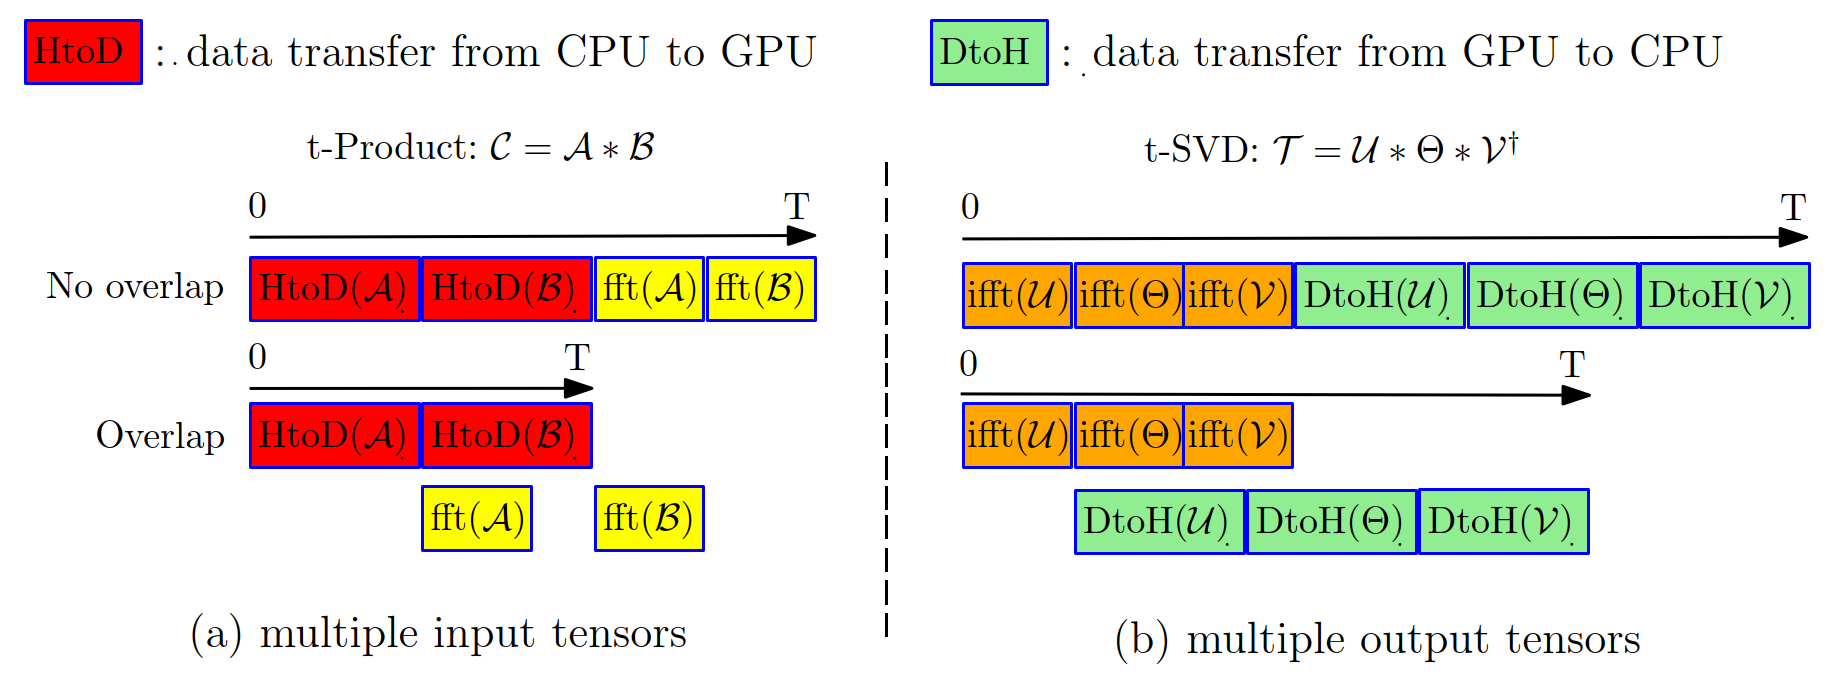
\includegraphics[width=\linewidth]{figs/cutensor_datatrans.png}\\
	Overlapping data transfer with computations
	\label{fig:cutensor_datatrans}
\end{figure}
\end{frame}

\begin{frame}{cuTensor-tubal (GPU)}
\framesubtitle{ Uniform Memory Access to Tube and Slice Data Structures}
\vskip -2ex
\vfill
\begin{figure}
	\centering  
	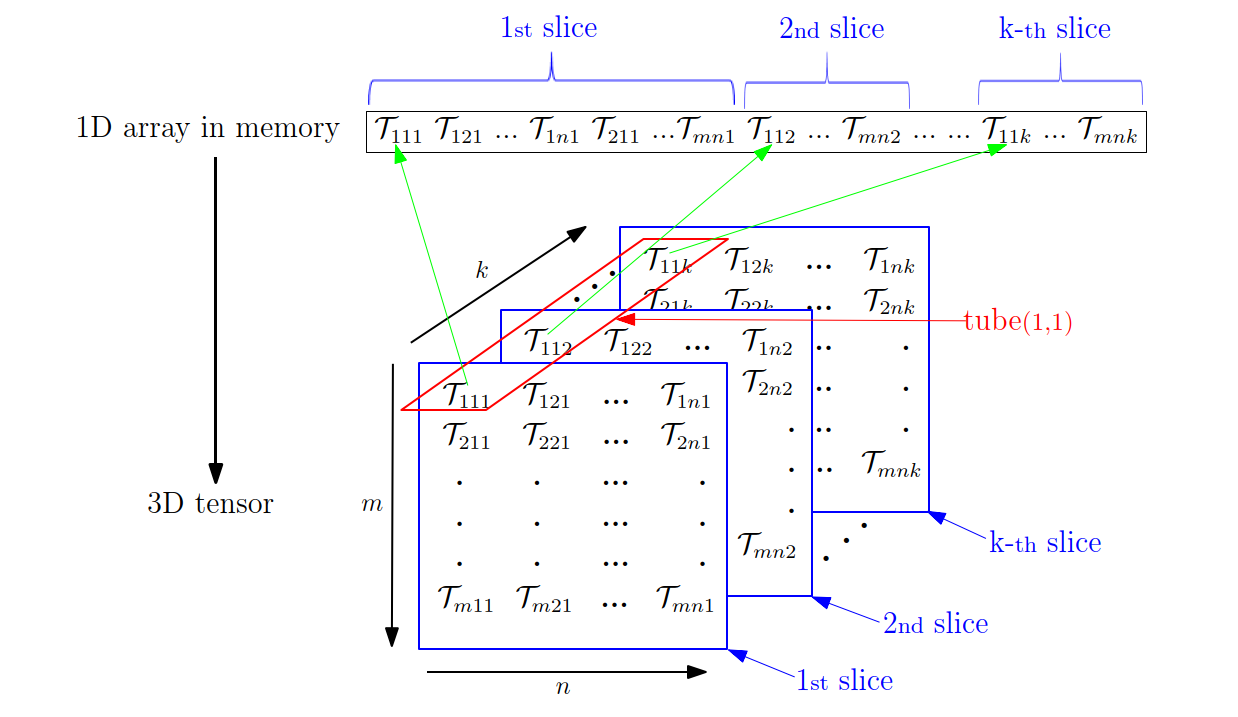
\includegraphics[width=0.5\linewidth]{figs/cutensor_datastorage.png}\hfill  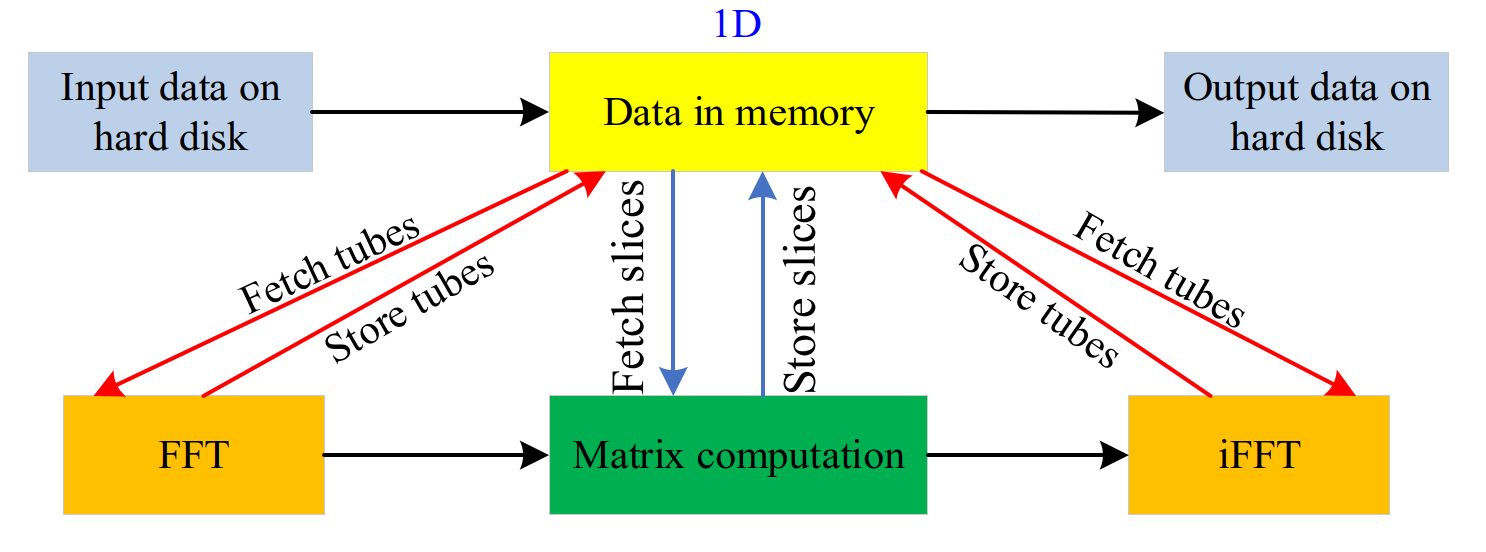
\includegraphics[width=0.5\linewidth]{figs/cutensor_datastructure.png}\\
	Tensors are stored as a 1D array in memory\hfill Data structures in tensor computations~~~~~
	\label{fig:cutensor_datastructure}
\end{figure}
\vfill
\end{frame}

\begin{frame}{cuTensor-tubal (GPU)}
\framesubtitle{Parallelizing the Fourier Transforms and Matrix Computations}

\begin{table}
$\begin{array}{l | l | l |l}
\textbf{Operation} & \textbf{\#(FFT operations)} & \textbf{\#(Matrix Operation)} & \textbf{\#(inverse FFT operation)}\\
\hline \hline
\text{t-FFT} & m \times n & \text{None} & m \times n \\
\text{inverse t-FFT} & m \times n & \text{None} & m \times n \\
\text{t-product} & m \times l + l\times n & k & m \times n \\
\text{t-SVD} & m \times n & k & m \times n + n\times n + m\times n \\
\text{t-QR} & m \times n & k & m \times m + m \times n \\
\text{t-inverse} & n \times n & k & n \times n \\
\text{t-normalization} & m & k & m 
\end{array}$
\caption{Seven tensor operations in the cuTensor-tubal library}
\end{table}
\end{frame}

\begin{frame}{cuTensor-tubal (GPU)}
\begin{figure}
	\centering  
	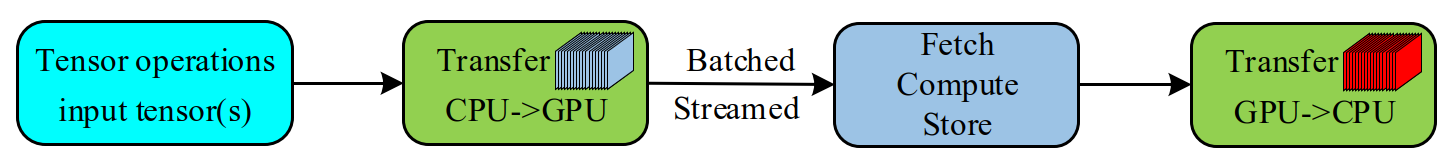
\includegraphics[width=0.9\linewidth]{figs/cutensor_workflow.png} \\
	System workflow of the cuTensor-tubal library
	\label{fig:cutensor_workflow}
\end{figure}
\begin{figure}
	\centering  
	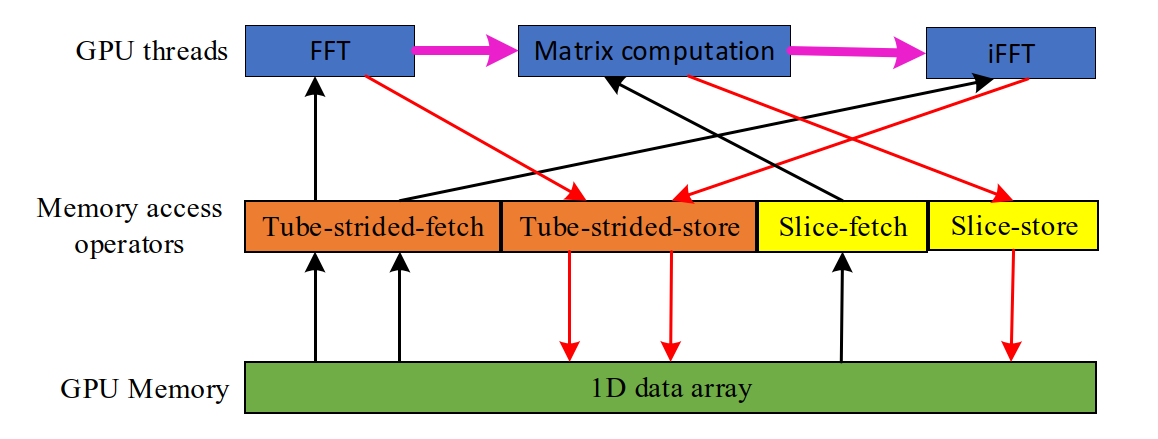
\includegraphics[width=0.6\linewidth]{figs/cutensor_memoryaccess.png} \\
	Memory access operators
	\label{fig:cutensor_memoryaccess}
\end{figure}
\end{frame}

\begin{frame}{TenDeC++ (CPU)}
\begin{columns}
\column{0.55\linewidth}
TenDeC++ is a new library for tensor decompositions in C++, in which a novel underlying technology \textbf{PointerDefomer} leveraging he unique pointer is proposed to further explore potentials of C++. TenDeC++ supports 
\begin{itemize}
\item Canonical Polyadic
\item Tucker Decomposition
\item Tensor-train Decomposition
\item t-SVD
\end{itemize}
Compared with Tensorly in Python and TensorLab in MATLAB, TenDeC++ reduces more than \textbf{83.7\%}, \textbf{53.3\%} decomposition time, and supports \textbf{2.5$\times$}, \textbf{2$\times$} of tensor.
\column{0.45\linewidth}
\vskip -2ex
\begin{figure}
	\centering  
	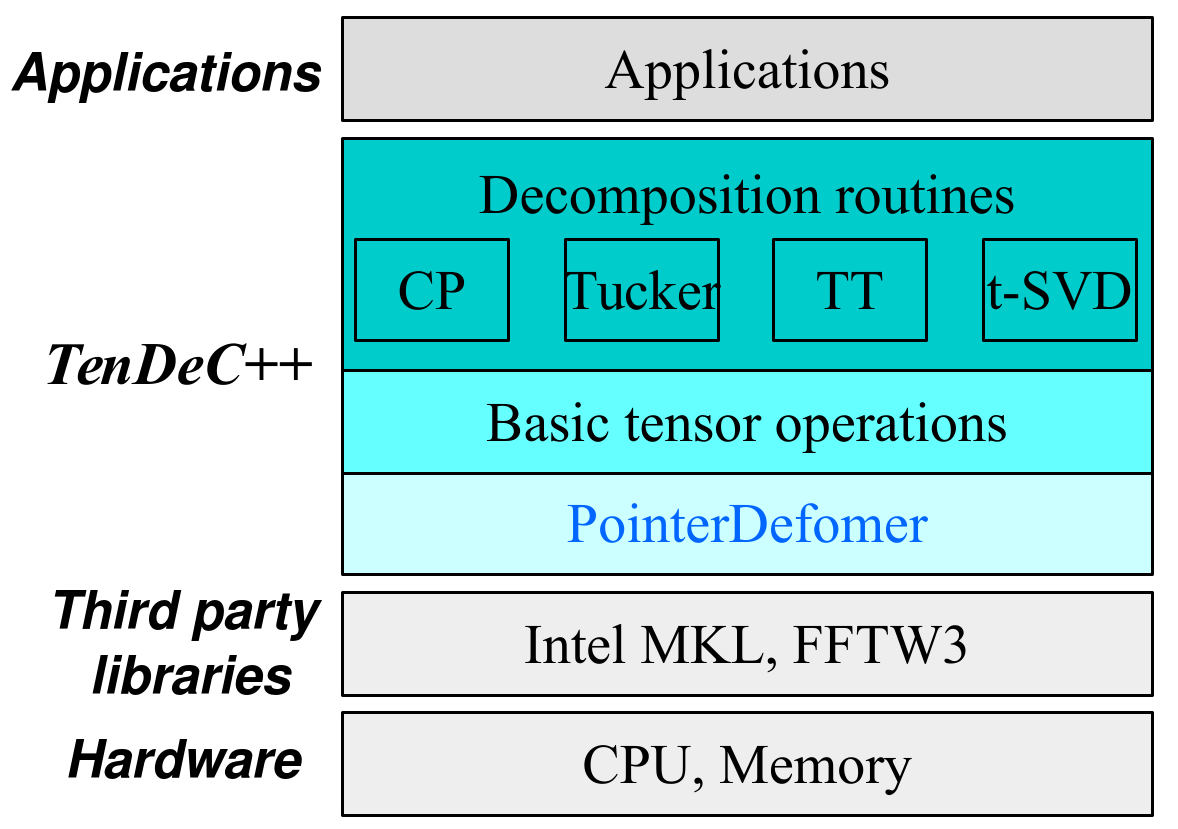
\includegraphics[width=\linewidth]{figs/tendecpp_arch.png} \\
	System architecture of the TenDeC++ library
	\label{fig:tendecpp_arch}
\end{figure}
\end{columns}
\vfill
\end{frame}

\begin{frame}{TenDeC++ (CPU)}
\framesubtitle{PointerDeformer}
A 3D tensor is stored as a 1D array in memory. Accessing these data with different sequences can form size-specific matrices including three mode-$n$ views: column-major, row-major, and concatenation views. These virtual views motivate us to design PointerDeformer to skip the time-consuming unfolding operation in C++.
\begin{figure}
	\centering  
	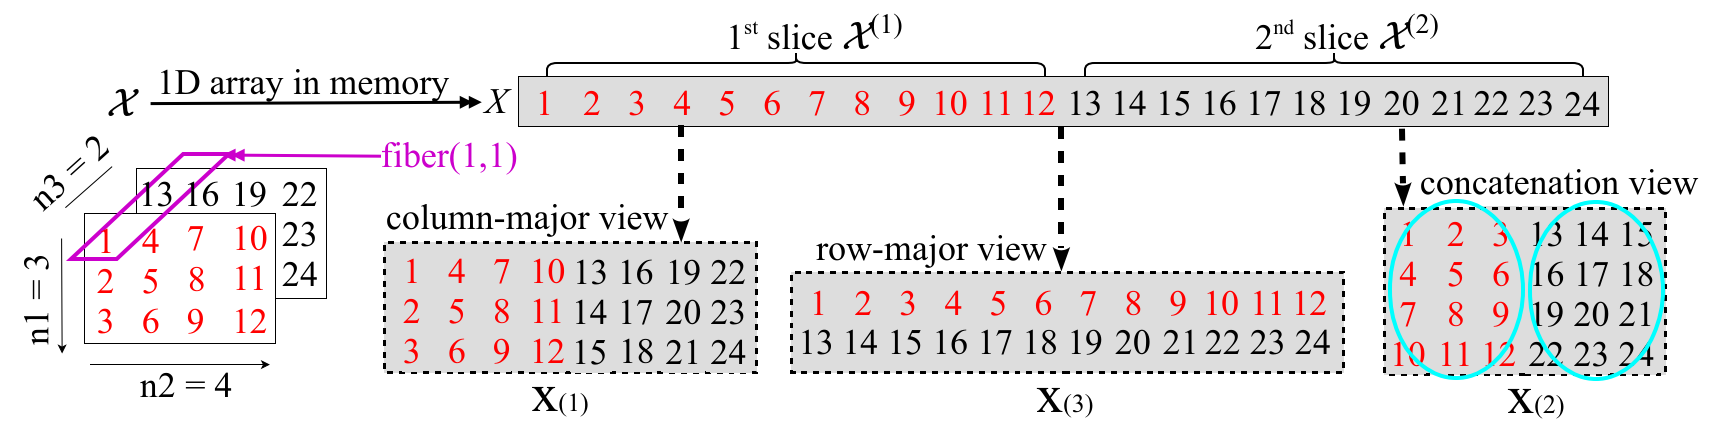
\includegraphics[width=\linewidth]{figs/pointerdeformer_example.png}
	\label{fig:pointerdeformer_example}
\end{figure}
\end{frame}

\begin{frame}{TenDeC++ (CPU)}
\framesubtitle{Optimized Basic Tensor Operation: $n$-mode Product}
Compare with traditional process, the optimized process does not need the time-consuming unfold/fold operations. Instead, PointerDeformer achieves the virtual transformation by accessing the data with specific sequence in memory.
\begin{figure}
	\centering  
	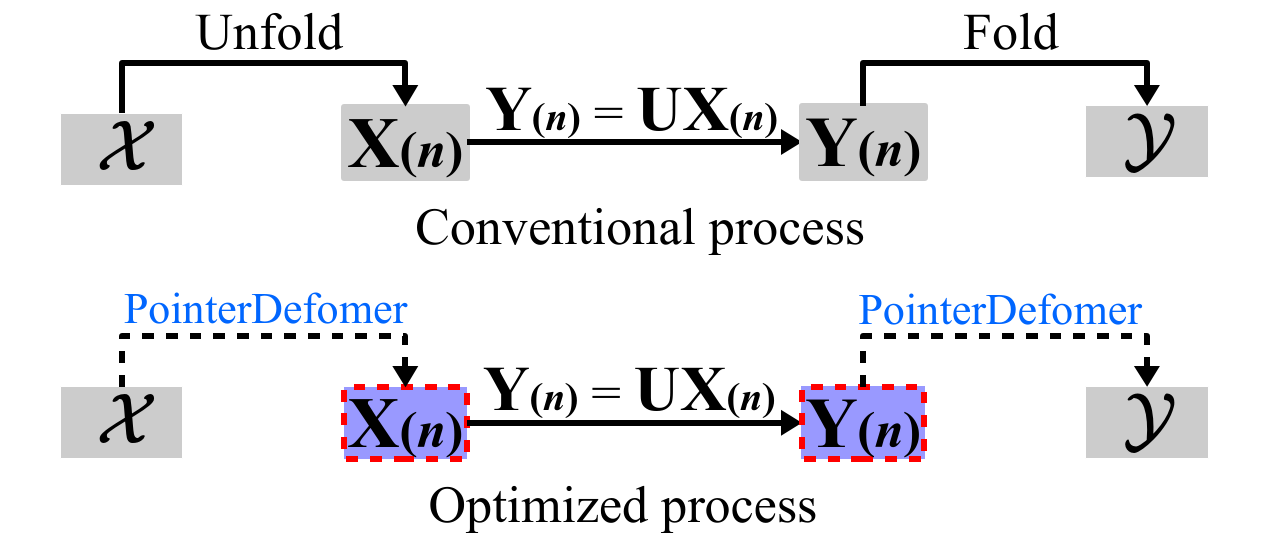
\includegraphics[width=0.6\linewidth]{figs/tendecpp_optimized.png}
	\label{fig:tendecpp_optimized}
\end{figure}
\end{frame}

\begin{frame}{TenDeC++ (CPU)}
\framesubtitle{Other Acceleration Techniques}
\large
\begin{itemize}
\item Exploit Symmetry with PointerDefomer
\item Exploit Conjugate Symmetry for t-SVD Decomposition
\normalsize
\vskip 1ex
Based on the conjugate symmetric property of FFT for real input data, there is $\texttt{conj}(\hat{\mathcal{X}}^{(j)})=\hat{\mathcal{X}}^{(k-j+2)}$, where $j=2,3,\cdots,\lceil\frac{k+1}{2}\rceil$ and $\texttt{conj}(\mathbf{X})$ denotes the conjugate of matrix $\mathbf{X}$. Conjugation on both sides of $\hat{\mathcal{X}}^{(j)}=\hat{\mathcal{U}}^{(j)}\hat{\mathcal{S}}^{(j)}\hat{\mathcal{V}}^{(j)}$,
$$
\hat{\mathcal{X}}^{(k-j+2)}=\texttt{conj}(\hat{\mathcal{U}}^{(j)})\cdot\texttt{conj}(\hat{\mathcal{S}}^{(j)})\cdot\texttt{conj}(\hat{\mathcal{V}}^{(j)}).
$$
Hence, with the conjugate symmetry, it only needs to preform SVD on \textbf{half} slice in t-SVD decomposition.
\end{itemize}
\end{frame}

\begin{frame}{TenDeC++ (CPU)}
\framesubtitle{Performance}
\vskip -4.6ex
\begin{columns}
\column{0.5\linewidth}
\begin{figure}
	\centering  
	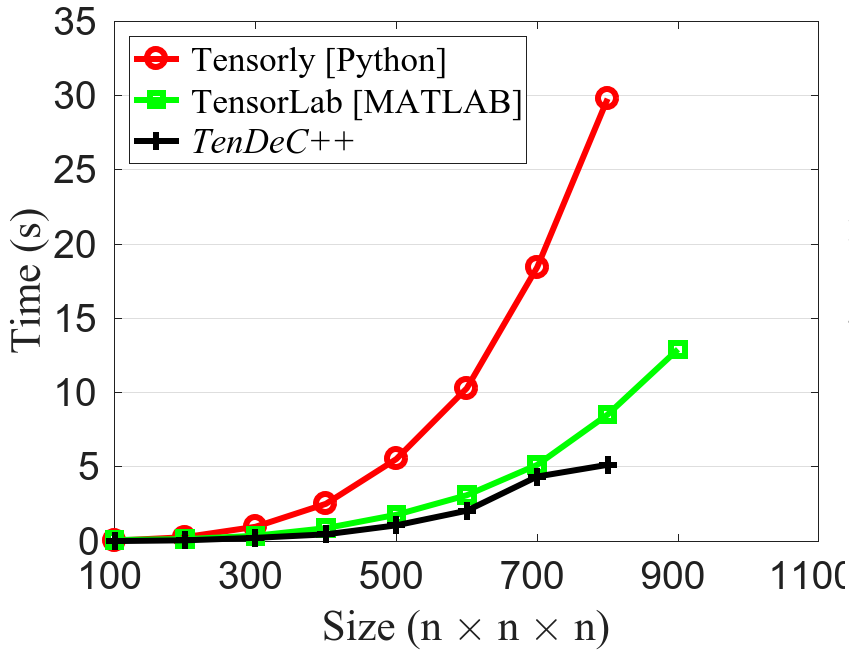
\includegraphics[width=\linewidth]{figs/tendecpp_eval3.png}\\
	Running time of CP decomposition
	\label{fig:tendecpp_eval1}
\end{figure}
\column{0.5\linewidth}
\vskip -0.6ex
\begin{figure}
	\centering  
	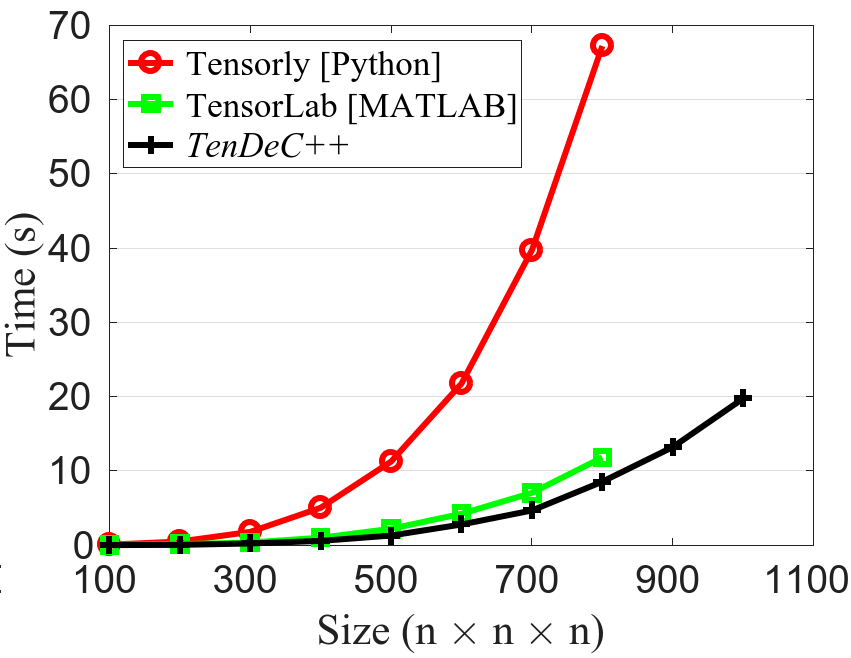
\includegraphics[width=\linewidth]{figs/tendecpp_eval1.png}\\
	Running time of Tucker decomposition
	\label{fig:tendecpp_eval2}
\end{figure}
\end{columns}
\end{frame}

\begin{frame}{TenDeC++ (CPU)}
\framesubtitle{Performance}
\begin{figure}
	\centering  
	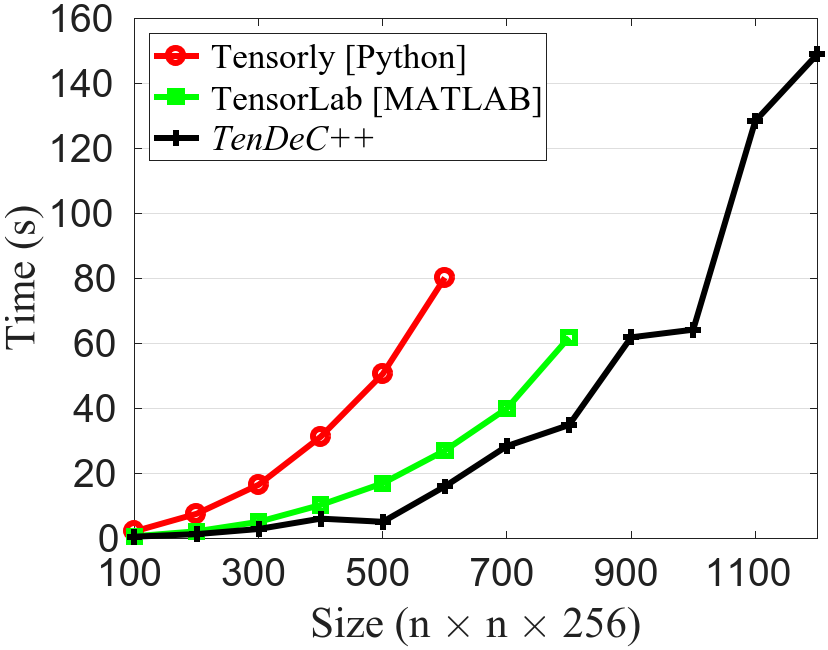
\includegraphics[width=0.5\linewidth]{figs/tendecpp_eval2.png}\\
	Running time of t-SVD
	\label{fig:tendecpp_eval3}
\end{figure}
\end{frame}
\end{document}
